\chapter{Indexed methods}
\label{chr:index}

Suffix trees are elegant data structures but they are rarely used in practice.
Although suffix trees provides theoretically optimal construction and query time, their high space consumption prohibits practical indexing of large string collections.
A practical study on suffix trees by \cite{Kurtz1999} reports that efficient implementations achieve sizes between $12\Slen$ and $20\Slen$ bytes per character.
For instance, two years before completing the sequencing of the human genome, \citeauthor{Kurtz1999} conjectured the resources required for computing the suffix tree for the complete human genome (consisting of about $3 \cdot 10^9$~bp) in 45.31~GB of memory and nine hours of CPU time, and concluded that \emph{``it seems feasible to compute the suffix tree for the entire human genome on some computers''}.

One might be tempted to think that such memory requirements are not anymore a limiting factor as, at the time of writing, even standard workstations come with 32~GB of main memory.
Indeed, over the last decades, the semiconductors industry followed the exponential trends dictated by Moores' law and yielded not only exponentially faster microprocessors but also larger memories.
Unfortunately, memory latency improvements have been more modest, leading to the so called memory wall effect \citep{Wilkes1995}: data access times are taking an increasingly fraction of total computation times.
Thus, if \cite{Knuth1973} wrote that \emph{``space optimization is closely related to time optimization in a disk memory''}, forty years later one can simply say that space optimization is always related to time optimization.

Over the last years, significant effort has been devoted to the engineering of more space-efficient data structures to replace the suffix tree in practical applications.
In particular, much research has been done into designing succinct (or even compressed) data structures providing efficient query times using space proportional to that of the uncompressed (or compressed) input.
Thanks to these advances, a succinct index of the human genome consumes as little as 3.5~GB of memory and often even improves query time over classic indices.

In this chapter, I introduce some classic full-text indices (suffix arrays and $q$-gram indices) and subsequently succinct full-text indices (uncompressed variants of the FM-index).
Afterwards, I introduce generic string matching algorithms that work on any of these data structures, and at the same time provide their experimental evaluation.
My implementation of all these algorithms and data structures is publicly available in source form within the \CC library SeqAn \citep{Doering2008}.

\section{Classic full-text indices}

\subsection{Suffix array}
\label{sec:index:sa}

The suffix array (SA) has been initially proposed by \cite{Manber1990} as a practical replacement of the suffix tree in exact string matching.
The SA reduces the space complexity of the suffix tree by a constant factor at the cost of an increase of the search time complexity by a logarithmic factor.
It achieves that by explicitly representing only the leaves of the suffix trie while omitting its internal nodes and outgoing edges.
Figure~\ref{fig:sa_gsa} shows an example.
The leaves referring to sorted suffixes are sufficient to emulate suffix trie traversals.
Any path from the root to some internal node is indeed computed on the fly via binary search over the sorted suffixes.
Below, I define the (generalized) suffix array and then show how to emulate all top-down traversal operations.

\begin{definition}[Suffix array]
The \emph{suffix array} of a padded string $\String$ of length $\Slen$ is an array $\Sarray$ containing a permutation of the interval $\OInterval{\At{1}}{\Slen}$, \st $\Suffix{\String}{\SubscriptNV{\Sarray}{i-1}} \lexlt \Suffix{\String}{\SubscriptNV{\Sarray}{i}}$ for all $\At{2} \leq i \LeqThan{\Slen}$.
\end{definition}

\begin{definition}[Generalized suffix array]
The \emph{generalized suffix array} (GSA) of a padded string collection $\Strings$ (definition~\ref{def:coltd}), consisting of $\Scard$ strings of total length $\Slen$, is an array $\Sarray$ of length $\Slen$ containing a permutation of all pairs $(i,j)$ with $\At{1} \leq i \LeqThan{\Scard}$ and $\At{1} \leq j \LeqThan{|\AtCollection{\String}{i}|}$.
Pairs are ordered \st $\Suffix{\Strings}{\SubscriptNV{\Sarray}{i-1}} \lexlt \Suffix{\Strings}{\SubscriptNV{\Sarray}{i}}$ for all $\At{2} \leq i \LeqThan{\Slen}$.
\end{definition}

\begin{figure}[b]
\label{fig:sa_gsa}
\begin{center}
\caption[Example of (generalized) suffix array]{(Generalized) suffix array. (\subref{fig:sa}) Suffix array of the string {\ttfamily ANANAS\$}. (\subref{fig:gsa}) Generalized suffix array of the string collection $\Strings = \{$ {\ttfamily ANANAS$\AtCollection{\$}{\At{1}}$}, {\ttfamily CACAO$\AtCollection{\$}{\At{2}}$} $\}$.}

\begin{subfigure}[t]{0.45\textwidth}
\begin{center}
\caption[Example of suffix array]{Suffix array.}
\label{fig:sa}
\ttfamily
\begin{tabular}{ccl}
$i$ & $\SubscriptNV{\Sarray}{i}$ & $\Suffix{\String}{\SubscriptNV{\Sarray}{i}}$\\
\midrule
$\At{1}$ & $\At{7}$ & \$\\
$\At{2}$ & $\At{1}$ & ANANAS\$\\
$\At{3}$ & $\At{3}$ & ANAS\$\\
$\At{4}$ & $\At{5}$ & AS\$\\
$\At{5}$ & $\At{2}$ & NANAS\$\\
$\At{6}$ & $\At{4}$ & NAS\$\\
$\At{7}$ & $\At{6}$ & S\$\\
\end{tabular}
\end{center}
\end{subfigure}%
\begin{subfigure}[t]{0.45\textwidth}
\begin{center}
\caption[Example of generalized suffix array]{Generalized suffix array.}
\label{fig:gsa}
\ttfamily
\begin{tabular}{rcl}
$i$ & $\SubscriptNV{\Sarray}{i}$ & $\Suffix{\Strings}{\SubscriptNV{\Sarray}{i}}$\\
\midrule
$\At{1}$ & $(\At{1},\At{7})$ & $\AtCollection{\$}{\At{1}}$\\
$\At{2}$ & $(\At{2},\At{6})$ & $\AtCollection{\$}{\At{2}}$\\
$\At{3}$ & $(\At{2},\At{2})$ & ACAO$\AtCollection{\$}{\At{2}}$\\
$\At{4}$ & $(\At{1},\At{1})$ & ANANAS$\AtCollection{\$}{\At{1}}$\\
$\At{5}$ & $(\At{1},\At{3})$ & ANAS$\AtCollection{\$}{\At{1}}$\\
$\At{6}$ & $(\At{2},\At{4})$ & AO$\AtCollection{\$}{\At{2}}$\\
$\At{7}$ & $(\At{1},\At{5})$ & AS$\AtCollection{\$}{\At{1}}$\\
$\At{8}$ & $(\At{2},\At{1})$ & CACAO$\AtCollection{\$}{\At{2}}$\\
$\At{9}$ & $(\At{2},\At{3})$ & CAO$\AtCollection{\$}{\At{2}}$\\
$\At{10}$ & $(\At{1},\At{2})$ & NANAS$\AtCollection{\$}{\At{1}}$\\
$\At{11}$ & $(\At{1},\At{4})$ & NAS$\AtCollection{\$}{\At{1}}$\\
$\At{12}$ & $(\At{2},\At{5})$ & O$\AtCollection{\$}{\At{2}}$\\
$\At{13}$ & $(\At{1},\At{6})$ & S$\AtCollection{\$}{\At{1}}$\\
\end{tabular}
\end{center}
\end{subfigure}

\end{center}
\end{figure}

The SA is constructed in $\Oh(\Slen)$ time, for instance using the \citep{Kaerkkaeinen2003} algorithm, or using non-optimal but practically faster algorithms, \eg \citep{Schuermann2007}.
The space consumption of the SA is $\Slen \log{\Slen}$ bits.
When $\Slen < 2^{32}$, a 32 bit integer is sufficient to encode any value in the range $\OInterval{\At{1}}{\Slen}$.
Consequently, the space consumption of suffix arrays for strings shorter than 4~GB is $4 \Slen$ bytes.

\cite{Weese2013} gives a generalization of \citeauthor{Kaerkkaeinen2003} algorithm to construct the GSA in $\Oh(\Slen)$ time.
The space consumption of the GSA is $\Slen \log{\AtCollection{\Slen}{*}}$ bits, where $\AtCollection{\Slen}{*} = \max{\,\AtCollection{\Slen}{i}}$.
For instance, for collections consisting of not more than 256 strings shorter than 4~GB in total, a pair of $1+4$~bytes suffices to encode any suffix position.

\begin{figure*}[t!]
\begin{minipage}[t]{.5\textwidth}
\begin{algorithm}[H]
\Algorithm{L}{$\StrieNode,\StrieChar$}
\begin{tabular}{ll}
\textbf{Input}  & $\StrieNode$ : SA node iterator\\
				& $\StrieChar$ : character to query\\
\textbf{Output} & integer denoting the left interval\\
\end{tabular}
\begin{algorithmic}[1]
\State {$(l_1,l_2) \gets (\StrieNode.l,\StrieNode.r)$}
\While {$l_1 < l_2$}
	\State {$i \gets \lfloor \frac{l_1+l_2}{2} \rfloor$}
	\If {$\Subscript{\Strings}{\SubscriptNV{\Sarray}{i} + \StrieNode.d} \lexlt \StrieChar$}
		\State {$l_1 \gets i+1$}
	\Else
		\State {$l_2 \gets i$}
	\EndIf
\EndWhile
\State \Return $l_1$
\end{algorithmic}
\label{alg:sa-lower}
\end{algorithm}
\end{minipage}
\hfill
\begin{minipage}[t]{.5\textwidth}
\begin{algorithm}[H]
\Algorithm{R}{$\StrieNode,\StrieChar$}
\begin{tabular}{ll}
\textbf{Input}  & $\StrieNode$ : SA node iterator\\
				& $\StrieChar$ : character to query\\
\textbf{Output} & integer denoting the right interval\\
\end{tabular}
\begin{algorithmic}[1]
\State {$(r_1,r_2) \gets (\StrieNode.l,\StrieNode.r)$}
\While {$r_1 < r_2$}
	\State {$i \gets \lfloor \frac{r_1+r_2}{2} \rfloor$}
	\If {$\Subscript{\Strings}{\SubscriptNV{\Sarray}{i} + \StrieNode.d} \lexleq \StrieChar$}
		\State {$r_1 \gets i+1$}
	\Else
		\State {$r_2 \gets i$}
	\EndIf
\EndWhile
\State \Return $r_1$
\end{algorithmic}
\label{alg:sa-upper}
\end{algorithm}
\end{minipage}
\end{figure*}

\subsubsection{Top-down traversal}

I now concentrate on describing suffix trie functionalities, as I implemented them within the SeqAn library.
Any suffix trie node is univocally identified by an interval of the suffix array $\Sarray$.
For instance, the root node is represented by the interval $\OInterval{\At{1}}{\Slen}$ containing the whole SA.
Thus, while traversing the trie, I remember the interval $\OInterval{l}{r}$ associated to the current node.
In addition, I also remember the right interval $r_p$ of the parent node and the depth $d$ of the current node.
The incoming edge label of an internal node at depth $d$ is identified by the $(\AtEnd{d})$-th symbol within the corresponding suffix $\Suffix{\Strings}{\SubscriptNV{\Sarray}{i}}$ with $i \in \OInterval{l}{r}$.
Any leaf node is defined to have all outgoing edges labeled by terminator symbols (see section~\ref{sub:introindex}).
The occurrences below any node correspond by definition to the interval $\OInterval{l}{r}$ of $\Sarray$.
Summing up, I represent the current node $\StrieNode$ by the integers $\{ l, r, r_p, d \}$ and define the following operations on it:
\begin{itemize}
\item \FunctionCall{goRoot}{\StrieNode} initializes $\StrieNode$ to $\{ \At{1}, \Slen, \Slen, 0\}$;
%\item \FunctionCall{isRoot}{\StrieNode} returns true iff $d = 0$;
\item \FunctionCall{isLeaf}{\StrieNode} returns true iff $|\Suffix{\Strings}{\SubscriptNV{\Sarray}{\AtEnd{\StrieNode.r}}}|=\StrieNode.d+1$
\item \FunctionCall{label}{\StrieNode} returns $\Subscript{\Strings}{\SubscriptNV{\Sarray}{\StrieNode.l} + \StrieNode.d}$;
\item \FunctionCall{occurrences}{\StrieNode} returns $\OSubstringNV{\Sarray}{\StrieNode.l}{\StrieNode.r}$.
\end{itemize}

\begin{figure*}[t!]
\begin{minipage}[t]{.5\textwidth}
\begin{algorithm}[H]
\Algorithm{goDown}{$\StrieNode$}
\begin{tabular}{ll}
\textbf{Input}  & $\StrieNode$ : SA node iterator\\
\textbf{Output} & boolean indicating success\\
\end{tabular}
\begin{algorithmic}[1]
\If {\Call{isLeaf}{$\StrieNode$}}
	\State \Return \False
\EndIf
\State {$\StrieNode.l \gets$ \Call{R}{$\StrieNode,\$$}}
\State {$\StrieChar_l \gets \Subscript{\Strings}{\SubscriptNV{\Sarray}{\StrieNode.l} + \StrieNode.d}$}
\State {$\StrieChar_r \gets \Subscript{\Strings}{\SubscriptNV{\Sarray}{\AtEnd{\StrieNode.r}} + \StrieNode.d}$}
\State {$\StrieNode.r_p \gets \StrieNode.r$}
\If {$\StrieChar_l \neq \StrieChar_r$}
	\State {$\StrieNode.r \gets$ \Call{R}{$\StrieNode,\StrieChar_l$}}
\EndIf
\State {$\StrieNode.d \gets \StrieNode.d+1$}
\State \Return \True
\end{algorithmic}
\label{alg:sa-godown}
\end{algorithm}
\end{minipage}
\hfill
\begin{minipage}[t]{.5\textwidth}
\begin{algorithm}[H]
\Algorithm{goRight}{$\StrieNode$}
\begin{tabular}{ll}
\textbf{Input}  & $\StrieNode$ : SA node iterator\\
\textbf{Output} & boolean indicating success\\
\end{tabular}
\begin{algorithmic}[1]
\If {$\StrieNode.r = \StrieNode.r_p$}
	\State \Return \False
\EndIf
\State {$\StrieNode.l \gets \StrieNode.r$}
\State {$\StrieChar_l \gets \Subscript{\Strings}{\SubscriptNV{\Sarray}{\StrieNode.l} + \StrieNode.d}$}
\State {$\StrieChar_r \gets \Subscript{\Strings}{\SubscriptNV{\Sarray}{\AtEnd{\StrieNode.r}} + \StrieNode.d}$}
\State {$\StrieNode.r \gets \StrieNode.r_p$}
\If {$\StrieChar_r \neq \StrieChar_p$}
	\State {$\StrieNode.r \gets$ \Call{R}{$\StrieNode,\StrieChar_r$}}
\EndIf
\State \Return \True
\item[]
\end{algorithmic}
\label{alg:sa-goright}
\end{algorithm}
\end{minipage}
\end{figure*}

Binary search is the key to implement function \FunctionName{goDown} a symbol.
Functions \FunctionName{L} (algorithm~\ref{alg:sa-lower}) and \FunctionName{R} (algorithm~\ref{alg:sa-upper}) compute in $\Oh(\log{\Slen})$ binary search steps the position in $\Sarray$ of the left and right intervals corresponding to the child node that is reached by going down the edge labeled by a given symbol $\StrieChar$.
Algorithms~\ref{alg:sa-godown} and \ref{alg:sa-goright} show how to implement respectively \FunctionName{goDown} and \FunctionName{goRight} with a time complexity independent of the alphabet size $\sigma$.
As they rely on a single call of \FunctionName{R}, their time complexity is $\Oh(\log{\Slen})$.
In this way, the SA supports exact string matching in $\Oh(\Plen \log{\Tlen})$ time (see algorithm~\ref{alg:st-exact}).

\begin{figure*}[b!]
\begin{center}
\begin{minipage}[t]{.6\textwidth}
\begin{algorithm}[H]
\Algorithm{goDown}{$\StrieNode,\StrieChar$}
\begin{tabular}{ll}
\textbf{Input}  & $\StrieNode$ : SA node iterator\\
				& $\StrieChar$ : character to query\\
\textbf{Output} & boolean indicating success\\
\end{tabular}
\begin{algorithmic}[1]
\If {\Call{isLeaf}{$\StrieNode$}}
	\State \Return \False
\EndIf
\State {$l \gets \Call{L}{\StrieNode,\StrieChar}$}
\State {$r \gets \Call{R}{\StrieNode,\StrieChar}$}
\If {$l < r$}
	\State {$\StrieNode \gets \{ l, r, \StrieNode.r, \StrieNode.d +1 \}$}
	\State \Return \True
\Else
	\State \Return \False
\EndIf
\end{algorithmic}
\label{alg:sa-godownc}
\end{algorithm}
\end{minipage}
\end{center}
\end{figure*}

Note that the suffix array can be binary searched by spelling a full pattern within a single call of \FunctionName{L} and \FunctionName{R}: in line 6 of algorithms~\ref{alg:sa-lower}--\ref{alg:sa-upper}, instead of comparing a single character, it suffices to compare the full pattern to the current suffix.
Nonetheless, the worst case runtime of algorithm~\ref{alg:st-exact} stays $\Oh(\Plen \log{\Tlen})$, as each step of the binary search requires a full lexicographical comparison between the pattern and any suffix of the text, which takes $\Oh(\Plen)$ time in the worst case.
As shown in \citep{Manber1990}, the worst case runtime can be decreased to $\Oh(\Plen + \log{\Tlen})$ at the expense of additional $\Tlen \log{\Tlen}$ bits, by storing the precomputed longest common prefixes (LCP) between any two consecutive suffixes $\Suffix{\Strings}{\SubscriptNV{\Sarray}{i}}$, $\Suffix{\Strings}{\SubscriptNV{\Sarray}{i+1}}$ for all $1 \leq i < \Slen$.
Alternatively, the \emph{average case} runtime is reduced to $\Oh(\Plen + \log{\Tlen})$, without storing any additional information, by using the MLR heuristic \citep{Manber1990}.
In practice, the MLR heuristic outperforms the SA + LCP algorithm, due to the higher cost of fetching additional data from the LCP table \citep{Weese2013}.
%Thus I replace algorithm~\ref{alg:st-exact} by algorithm~\ref{alg:sa-exact}.

%\begin{figure}[h]
%\begin{center}
%\caption[Exact string matching on a suffix array]{Exact string matching on a suffix array. The pattern NA is searched exactly in the text ANANAS.}
%\label{fig:sa-exact}
%%\begin{tikzpicture}[scale=1.5,font=\sf]

\tikzstyle{level 1}=[sibling distance=12mm, level distance=6mm]
\tikzstyle{level 2}=[sibling distance=6mm, level distance=6mm]
\tikzstyle{level 3}=[sibling distance=6mm, level distance=6mm] 
\tikzstyle{level 4}=[sibling distance=6mm, level distance=6mm] 
\tikzstyle{level 5}=[sibling distance=6mm, level distance=6mm] 
\tikzstyle{level 6}=[sibling distance=6mm, level distance=6mm] 
\tikzstyle{level 7}=[sibling distance=6mm, level distance=6mm] 

%\tikzstyle{transparent}=[edge from parent/.style={draw=none}]
%\tikzstyle{el}=[->,thick,color=gray,text=mycolor1high]

\tikzstyle{transparent}=[edge from parent/.style={draw=none}]
\tikzstyle{el}=[->,thick,color=black,text=black]
\tikzstyle{inner}=[circle,draw,color=black,inner sep=1.5pt]

\node[inner](r) {}
child[transparent] {
node[inner](A) {}
child[transparent] {
node[inner](AN) {}
child[transparent] {
node[inner](ANA) {}
child[transparent] {
node[inner](ANAN) {}
child[transparent] {
node[inner](ANANA) {}
child[transparent] {
node[inner](ANANAS) {}
child[transparent] {
node[leaf](ANANASD) {$1$}
}
}
}
}
child[transparent] {
node[inner](ANAS) {}
child[transparent] {
node[leaf](ANASD) {$3$}
}
}
}
}
child[transparent] {
node[inner](AS) {}
child[transparent] {
node[leaf](ASD) {$5$}
}
}
}
child[transparent] {
node[inner](N) {}
child[transparent] {
node[inner](NA) {}
child[transparent] {
node[inner](NAN) {}
child[transparent] {
node[inner](NANA) {}
child[transparent] {
node[inner](NANAS) {}
child[transparent] {
node[leaf](NANASD) {$2$}
}
}
}
}
child[transparent] {
node[inner](NAS) {}
child[transparent] {
node[leaf](NASD) {$4$}
}
}
}
}
child[transparent] {
node[inner](S) {}
child[transparent] {
node[leaf](SD) {$6$}
}
}
;

\draw[el] (r) -- (A) \labelA{A};
\draw[el] (A) -- (AN) \labelA{N};
\draw[el] (AN) -- (ANA) \labelA{A};
\draw[el] (ANA) -- (ANAN) \labelA{N};
\draw[el] (ANAN) -- (ANANA) \labelA{A};
\draw[el] (ANANA) -- (ANANAS) \labelA{S};
\draw[el] (ANANAS) -- (ANANASD) \labelA{\$};
\draw[el] (ANA) -- (ANAS) \labelA{S};
\draw[el] (ANAS) -- (ANASD) \labelA{\$};
\draw[el] (A) -- (AS) \labelA{S};
\draw[el] (AS) -- (ASD) \labelA{\$};

\draw[el] (r) -- (N) \labelA{N};
\draw[el] (N) -- (NA) \labelA{A};
\draw[el] (NA) -- (NAN) \labelA{N};
\draw[el] (NAN) -- (NANA) \labelA{A};
\draw[el] (NANA) -- (NANAS) \labelA{S};
\draw[el] (NANAS) -- (NANASD) \labelA{\$};
\draw[el] (NA) -- (NAS) \labelA{S};
\draw[el] (NAS) -- (NASD) \labelA{\$};
\draw[el] (r) -- (S) \labelA{S};
\draw[el] (S) -- (SD) \labelA{\$};

\end{tikzpicture}


%\end{center}
%\end{figure}

\subsection{Suffix tree realizations}
\label{sec:index:stree}

I briefly introduce two suffix tree realizations from the literature: the \emph{enhanced suffix array} (ESA) \citep{Abouelhoda2004} and the \emph{lazy suffix tree} (LST) \citep{Giegerich2003}.
These realizations explicitly implement or implicitly emulate a suffix tree rather than a suffix trie.
The string matching algorithms of section \ref{sec:index:algo} work on tries, yet any tree can be easily traversed as a trie.
%Here, I only show how to adapt the traversal of any tree as a trie.
The implementation of these data structures within SeqAn, equally generalized to multiple sequence, is due to \citeauthor{Weese2013}.
Hence, for an extensive illustration, the reader is invited to consult \citep{Weese2013}.

\subsubsection{Enhanced suffix array}
\label{sec:index:esa}

The enhanced suffix array (ESA) \citep{Abouelhoda2004} supplements the SA and LCP tables (see section \ref{sec:index:sa}) with another table called \emph{child} table.
Each SA value represents one leaf of the suffix tree, while each LCP value represent the length of one edge of the suffix tree.
What is still missing, in order to represent a full suffix tree, are the SA intervals of the children of each inner node.
These intervals would have to be computed in logarithmic time by \FunctionName{goRight} during a top-down SA traversal.
As proposed by \cite{Abouelhoda2004}, these intervals are computed in linear time, within one single bottom-up traversal, and stored in the child table, which consumes additional $\Slen \log \Slen$ bits, thus $4\Slen$ bytes for collections smaller than 4 GB.

\subsubsection{Lazy suffix tree}
\label{sec:index:lst}

The lazy suffix tree (LST) \citep{Giegerich1999} variant proposed by \citep{Weese2013} is composed by a partially sorted SA plus a node directory.
The SA initially reflects the ordering of the suffixes up to depth 1, and the node directory table contains only the root node.
During a top-down traversal, the current node at depth $i$ is expanded by means of the \emph{wotd} algorithm \citep{Giegerich1999}, which calls one round of radix sort to refine the ordering of the suffixes up to depth $i + 1$ and inserts the newly computed children nodes in the directory.
The construction of the full LST takes $\Oh(\Slen^2 + \sigma \Slen)$ time in the worst case.

\subsection{$q$-Gram index}
\label{sec:index:qgram}

If the traversal of the idealized suffix trie is bounded to a maximum depth $q$, the logarithmic factor paid by using the SA vanishes.
The idea is to supplement the SA with a so-called $q$-gram \emph{directory}: an additional array $D$ of $\sigma^q + 1$ integers that represent the SA ranges computed by algorithm~\ref{alg:sa-lower} for all possible words of length $q$ over $\Sigma$.

\begin{figure}[b!]
\begin{center}
\caption[Example of $q$-gram index]{$2$-Gram index of the string $\String = $ {\ttfamily ANANAS\$} over the alphabet $\Sigma = \{ \text{ {\ttfamily A}, {\ttfamily N}, {\ttfamily S} }\}$. The example shows the lookup of the $2$-gram {\ttfamily NA}. The hash value $h(\text{\ttfamily NA})=\At{4}$ addresses two lookups, respectively in $\SubscriptNV{D}{\At{4}}$ and $\SubscriptNV{D}{\At{5}}$, that in turn provide the range $\OInterval{\At{5}}{\At{7}}$ in $\Sarray$.} %Note that suffixes of $\String$ shorter than $q=2$ are disabled in $A$.}
\label{fig:qgram}
\ttfamily
\begin{tabular}{ccccccl}
$\Pattern$ & $h(\Pattern)$ & $\SubscriptNV{D}{h(\Pattern)}$ & \phantom{-} & $i$ & $\SubscriptNV{\Sarray}{i}$ & $\Suffix{\String}{\SubscriptNV{\Sarray}{i}}$\\
\midrule
AA & $\At{1}$ & $\At{2}$ & & $\cell{i1}{\At{1}}$ & $\cell{a1}{\At{7}}$ & \cell{s1}{\$}\\
AN & $\At{2}$ & $\At{2}$ & & $\At{2}$ & $\At{1}$ & ANANAS\$\\
AS & $\At{3}$ & $\At{4}$ & & $\At{3}$ & $\At{3}$ & ANAS\$\\
\cell{p}{NA} & \cell{h4}{$\At{4}$} & \cell{d5}{$\At{5}$} & & $\At{4}$ & $\At{5}$ & AS\$\\
NN & \cell{h5}{$\At{5}$} & \cell{d6}{$\At{7}$} & & \cell{i5}{$\At{5}$} & \cell{a5}{$\At{2}$} & NANAS\$\\
NS & $\At{6}$ & $\At{7}$ & & \cell{i6}{$\At{6}$} & \cell{a6}{$\At{4}$} & NAS\$\\
SA & $\At{7}$ & $\At{7}$ & & \cell{i7}{$\At{7}$} & \cell{a7}{$\At{6}$} & \cell{s7}{{S\$}}\\
SN & $\At{8}$ & $\At{7}$ \\
SS & $\At{9}$ & $\At{7}$ \\
   & $\At{10}$ & $\At{7}$ \\
\end{tabular}
%\around{p}
%\eround{h4}{h5}
%\eround{d5}{d6}
%\eround{i5}{i6}
\eround{a5}{a6}
\edge{p}{h4}
\edge{p}{h5}
\edge{h4}{d5}
\edge{h5}{d6}
\link{d5}{i5}
\link{d6}{i6}
%\strike{i1}{s1}
%\strike{i7}{s7}
\end{center}
\end{figure}

With the aim of addressing $q$-grams in the directory $D$, I impose a canonical code on $q$-grams through a bijective function $h : \Sigma^q \rightarrow \OInterval{\At{1}}{\sigma^q}$ defined as in \citep{Knuth1973}:
\begin{eqnarray}
%h(\Pattern) = 1 + \sum_{i=\At{1}}^{\AtEnd{q}}{\lexrank{\Subscript{\Pattern}{i}} \cdot \sigma^{q-i}} 	% 1-based
h(\Pattern) = \sum_{i=\At{1}}^{\AtEnd{q}}{\lexrank{\Subscript{\Pattern}{i}} \cdot \sigma^{q-i}}			% 0-based
\end{eqnarray}
where $\Pattern \in \Sigma^q$ is some $q$-gram and $\lexrank{}$ is the lexicographic rank defined on $\Sigma$ (see definition~\ref{def:rho}). 
% pose $\lexrank_0{c} = \lexrank{c} - 1$ 	% 1-based
The canonical code assigned by $h$ preserves the lexicographical ordering for all words not longer than $q$, \ie $\XSeq \lexlt \YSeq$ iff $h(\XSeq) < h(\YSeq)$ for all $\XSeq,\YSeq \in \Sigma^{\leq q}$.
The hash function $h$ allows to store in and retrieve from $D$ the left SA interval returned by algorithm~\ref{alg:sa-lower} for each $q$-gram, \ie $\SubscriptNV{D}{h(\Pattern)} = \FunctionCall{L}{\At{1},\Slen,\Pattern}$ for all $\Pattern \in \Sigma^q$.
Note that the right interval returned by algorithm~\ref{alg:sa-upper} is equivalent to the left interval of the following $q$-gram in lexicographical order and therefore available in $\SubscriptNV{D}{h(\Pattern)+1}$.

In practice, the $q$-gram index is applicable only to relatively small alphabets and tree depths.
For instance, parameters $\sigma = 4$ and $q=14$ imply a $q$-gram directory consisting of 268~M entries.
Using a 32 bits integer encoding, such directory alone consumes 1~GB of memory.

\subsubsection{Top-down traversal}

I now describe how I extended the SA traversal operations of section \ref{sec:index:sa} to use the $q$-gram directory $D$ within the generic text indexing framework of the SeqAn library.
Again, while traversing the trie, I maintain the current range $\OInterval{l}{r}$ and the current depth $d$.
In addition, I maintain the interval $\OInterval{l_h}{r_h}$ in $D$ and the incoming edge label $e$ node in order to answer \FunctionCall{label}{\StrieNode}.
Summing up, I represent the current node $\StrieNode$ by the elements $\{ l, r, d, l_h, r_h, e \}$.
I define the basic node operations as follows:
\begin{itemize}
\item \FunctionCall{goRoot}{\StrieNode} initializes $\StrieNode$ to $\{ \At{1}, \Slen, 0, \At{1}, \sigma^q, \epsilon \}$;
\item \FunctionCall{isLeaf}{\StrieNode} returns true iff $\StrieNode.d=q$;
\item \FunctionCall{label}{\StrieNode} returns $\StrieNode.e$;
\item \FunctionCall{occurrences}{\StrieNode} returns $\OSubstringNV{\Sarray}{\StrieNode.l}{\StrieNode.r}$.
\end{itemize}

\begin{figure*}[b!]
\begin{minipage}[b]{.5\textwidth}
\begin{algorithm}[H]
\Algorithm{L}{$\StrieNode,\StrieChar$}
\begin{tabular}{ll}
\textbf{Input}  & $\StrieNode$ : $q$-gram index iterator\\
				& $\StrieChar$ : character to query\\
\textbf{Output} & integer denoting the left interval\\
\end{tabular}
\begin{algorithmic}[1]
\State {$\StrieNode.l_h \gets \StrieNode.l_h + \lexrank{c} \cdot \sigma^{\StrieNode.d} $}
\State \Return $\SubscriptNV{D}{\StrieNode.l_h}$
\end{algorithmic}
\label{alg:qgram-lower}
\end{algorithm}
\end{minipage}
\hfill
\begin{minipage}[b]{.5\textwidth}
\begin{algorithm}[H]
\Algorithm{R}{$\StrieNode,\StrieChar$}
\begin{tabular}{ll}
\textbf{Input}  & $\StrieNode$ : $q$-gram index iterator\\
				& $\StrieChar$ : character to query\\
\textbf{Output} & integer denoting the right interval\\
\end{tabular}
\begin{algorithmic}[1]
\State {$\StrieNode.r_h \gets \StrieNode.r_h - \lexrank{\StrieChar} \cdot \sigma^{\StrieNode.d}$}
\State \Return $\SubscriptNV{D}{\StrieNode.r_h}$
\end{algorithmic}
\label{alg:qgram-upper}
\end{algorithm}
\end{minipage}
\end{figure*}

Algorithms \ref{alg:qgram-lower} and \ref{alg:qgram-upper} show respectively functions \FunctionName{L} and \FunctionName{R} using the directory $D$ instead of $\Sarray$.
In this way, both variants of \FunctionName{goDown} (algorithms \ref{alg:sa-godownc} and \ref{alg:sa-godown}) and \FunctionName{goRight} (algorithm \ref{alg:sa-goright}) take $\Oh(1)$ time.
Conversely, \FunctionName{goDown} and \FunctionName{goRight} are implemented by the generic algorithms \ref{alg:st-godown} and \ref{alg:st-goright} running in time $\Oh(\sigma)$.

\begin{figure*}[t]
\begin{center}
\begin{minipage}[t]{.6\textwidth}
\begin{algorithm}[H]
\Algorithm{goDown}{$\StrieNode,\StrieChar$}
\begin{tabular}{ll}
\textbf{Input}  & $\StrieNode$ : $q$-gram index iterator\\
				& $\StrieChar$ : character to query\\
\textbf{Output} & boolean indicating success\\
\end{tabular}
\begin{algorithmic}[1]
\If {\Call{isLeaf}{$\StrieNode$}}
	\State \Return \False
\EndIf
\State {$\StrieNode.d \gets \StrieNode.d+1$}
\State {$\StrieNode.e \gets \StrieChar$}
\State {$\StrieNode.l \gets \Call{L}{\StrieNode,\StrieNode.e}$}
\State {$\StrieNode.r \gets \Call{R}{\StrieNode,\StrieNode.e}$}
\State \Return $\StrieNode.l < \StrieNode.r$
\end{algorithmic}
\label{alg:qgram-godownc}
\end{algorithm}
\end{minipage}
\end{center}
\end{figure*}

%Exact string matching algorithm~\ref{alg:st-exact} runs in time $\Oh(q)$, nonetheless it can be improved to perform $\Oh(1)$ lookups in $D$.
%It suffices to compute the canonical code of the pattern in one step, as shown in algorithm~\ref{alg:qgram-exact}.

%\begin{center}
%\begin{minipage}[t]{.8\textwidth}
%\begin{algorithm}[H]
%\Algorithm{ExactSearch}{$t,p$}
%\begin{tabular}{ll}
%\textbf{Input}  & $\Text$ : pointer to the root node of the $q$-gram index of the text\\
%				& $p$ : string to query\\
%\textbf{Output} & list of all occurrences of the pattern in the text\\
%\end{tabular}
%\begin{algorithmic}[1]
%\State {$l \gets D[h(\Pattern)]$}
%\State {$r \gets D[h(\Pattern) + 1]$}
%\State \Report $\Sarray[l \dots r]$
%\end{algorithmic}
%\label{alg:qgram-exact}
%\end{algorithm}
%\end{minipage}
%\end{center}

The directory $D$ alone is sufficient for top-down traversals bounded to a maximum depth $q$;
the suffix array $\Sarray$ is accessed only to locate text locations pointed by the leaves.
In this case, the total ordering of the text suffixes in the SA can be relaxed to prefixes of length $q$.
This gives a twofold advantage, as one can
\begin{inparaenum}[(i)]
\item construct the SA more efficiently using bucket sorting and
\item maintain leaves in each bucket sorted by their relative text positions.
\end{inparaenum}
The latter property allows to compress the SA bucket-wise \eg using Elias $\delta$ encoding \citep{Elias1975} or to devise cache-oblivious strategies to process the occurrences \citep{Hach2010}.

The directory $D$ is still usable, even if the traversal needs to go below depth $q$.
An hybrid traversal can use the directory $D$ up to depth $q$ and later continue with binary searches on the suffix array $\Sarray$.
This hybrid traversal cuts the most expensive binary searches and increases memory locality.
Furthermore, this traversal becomes useful whenever the SA is too big to fit in main memory and has to reside in external memory.
In section \ref{sec:index:algo}, I show the experimental evaluation of this hybrid $q$-gram index.

\subsection{Trie and radix tree realizations}
\label{sec:index:trie}

Before turning to succinct full-text indices, I briefly describe how I reused the text-indices just exposed to implement tries and radix trees in the SeqAn library.
A trie is easily emulated by means of a partial SA.
I index only the first suffix of each string in the collection and subsequently construct the SA-based trie via quicksort in time $\Oh(\Slen \log{\Slen})$, where $\Slen$ is the total length of the string collection.
The top-down traversal based on binary search still works as described in section \ref{sec:index:sa}.
This trie is also extendable by a $q$-gram directory as in section \ref{sec:index:qgram}.
A radix tree is constructed in an analogous way, starting from the LST of section \ref{sec:index:lst}.
I fill the LST's partial SA as described above and subsequently apply the \emph{wotd} algorithm \citep{Giegerich1999} to construct the radix tree in time $\Oh(\sigma \Slen)$.


\section{Succinct full-text indices}

The \emph{Burrows-Wheeler transform} (BWT) \citep{Burrows1994} is a transformation defining a permutation of an input string.
Such transformation exposes two important properties: it is \emph{reversible} and it tends to produce \emph{runs of equal characters}.
The former property allows to recover the original string from its BWT alone, while the latter property makes the transformed string more amenable to compression.
Because of these two properties, the BWT is a fundamental method for text compression.
%and is practically used in the bzip2 tool \citep{Seward1996}.

Some years after its introduction, \citeauthor{Ferragina2000} proposed the BWT for full-text indexing.
They show in \citep{Ferragina2000} that the BWT allows to perform exact string matching and engineer in \citep{Ferragina2001} a compressed full-text index called FM-index.
Over the last years, the FM-index has been widely employed under different re-implementations by many popular bioinformatics tools \eg Bowtie \citep{Langmead2009} and BWA \citep{Li2009}, and is now considered a fundamental method for the indexing of genomic sequences.

In the following, I give the fundamental ideas behind the BWT.
Subsequently, I discuss my generalized FM-index implementation covering strings and string collections.

\subsection{Burrows-Wheeler transform}
\label{sec:index:bwt}

Let $\String$ be a padded string (definition~\ref{def:strd}) of length $\Slen$ over $\Sigma_{\$}$.
In the following, consider the string $\String$ to be \emph{cyclic} and its subscript $\Subscript{\String}{i}$ to be \emph{modular}, \ie $\Subscript{\String}{i} = \Subscript{\String}{i \imod{\Slen}}$ for any $i \in \Z$.
\begin{definition}[BWT]
\label{def:bwt}
Given a string $\String$ and its SA $\Sarray$, the BWT $\Last$ of $\String$ is a string over $\Sigma_{\$}$ with $\Subscript{\Last}{i}=\Subscript{\String}{\SubscriptNV{\Sarray}{i}-1}$.
\end{definition}

\begin{figure}[t]
\begin{center}
\caption[Example of Burrows-Wheeler transform]{Cyclic shifts matrix of the string $\String =$ {\ttfamily ANANAS\$}. Column $\Subscript{\String}{\SubscriptNV{\Sarray}{i}-1}$ is the BWT of $\String$.}
\label{fig:bwt}
\ttfamily
\begin{tabular}{cccccc}
$i$ & $\SubscriptNV{\Sarray}{i}$ & \phantom{-} & $\Subscript{\String}{\SubscriptNV{\Sarray}{i}}$ & $\dots$ & $\Subscript{\String}{\SubscriptNV{\Sarray}{i}-1}$\\
\midrule
$\At{1}$ & $\At{7}$ & & \$& ANANA  & \cell{l1}{S}\\
$\At{2}$ & $\At{1}$ & & A & NANAS  & \$\\
$\At{3}$ & $\At{3}$ & & A & NAS\$A & N\\
$\At{4}$ & $\At{5}$ & & A & S\$ANA & N\\
$\At{5}$ & $\At{2}$ & & N & ANAS\$ & A\\
$\At{6}$ & $\At{4}$ & & N & AS\$AN & A\\
$\At{7}$ & $\At{6}$ & & S & \$ANAN & \cell{l7}{\Sarray}\\
\end{tabular}
\eround{l1}{l7}
\end{center}
\end{figure}

To visualize the BWT, consider the square matrix consisting of all cyclic shifts of the string $\String$ sorted in lexicographical order. %where the $i$-th cyclic shift has the form $\Substring{\String}{i}{\Slen} \Prefix{\String}{i-1}$.
Note how the cyclic shifts matrix is related to the suffix array $\Sarray$ of $\String$: the $i$-th cyclic shift is $\Substring{\String}{\SubscriptNV{\Sarray}{i}}{\Slen} \Prefix{\String}{\SubscriptNV{\Sarray}{i-1}}$.
% (except when $\SubscriptNV{\Sarray}{i} = \Ibase$).
The BWT is the string obtained by concatenating the symbols in the last column of the sorted cyclic shifts matrix of $\String$.
Figure~\ref{fig:bwt} shows an example.

Note that the BWT easily generalizes to string collections.
Indeed, definition~\ref{def:bwt} still holds for a padded string collection $\Strings$ (definition~\ref{def:coltd}) and its cyclic shifts matrix sorted in lexicographical order.


The cyclic shifts matrix is conceptual and does not have to be constructed explicitly to derive the BWT of $\String$.
The BWT can be obtained in linear time by scanning the SA $\Sarray$ and assigning the symbol $\Subscript{\String}{\SubscriptNV{\Sarray}{i}-1}$ to the $i$-th BWT symbol.
However, constructing the BWT from the SA is not desirable in practice, especially for strings over small alphabets like DNA, as the SA consumes $\Slen \log{\Slen}$ bits in addition to the $\Slen \log{\sigma}$ bits of the BWT.
Therefore, some direct BWT construction algorithms working within $o(\Slen \log{\sigma})$ bits plus constant space have been recently proposed in \citep{Bauer2013, Crochemore2013}.

\begin{figure}[b]
\begin{center}
\caption[Example of functions $LF$ and $\Psi$]{Functions $LF$ and $\Psi$ of the string $\String = $ {\ttfamily ANANAS\$}. The example shows that $LF = \Psi^{-1}$, \eg $LF(\Psi(5)) = 5$ and $\Psi(LF(3)) = 3$. Moreover, the example shows that the relative order of characters between $\Last$ and $\First$ is preserved, \eg the first occurrence of $N$ in $\Last$ corresponds to the first occurrence in $\First$.}
\label{fig:lf_psi}
\ttfamily
\begin{tabular}{ccccccc}
$i$ & $\Psi(i)$ & $LF(i)$ & \phantom{-} & $\Subscript{\String}{\SubscriptNV{\Sarray}{i}}$ & $\dots$ & $\Subscript{\String}{\SubscriptNV{\Sarray}{i}-1}$\\
\midrule
$\At{1}$ & $\At{2}$ & $\At{7}$                        & & \$           & ANANA  & S\\
$\At{2}$ & $\At{5}$ & $\At{1}$                        & & A            & NANAS  & \$\\
$\At{3}$ & $\At{6}$ & \cell{lf3}{$\At{5}$} & & A      & NAS\$A & \cell{l3}{N}\\
$\At{4}$ & $\At{7}$ & $\At{6}$                        & & A            & S\$ANA & N\\
$\At{5}$ & \cell{psi5}{$\At{3}$} & $\At{2}$           & & \cell{f5}{N} & ANAS\$ & A\\
$\At{6}$ & $\At{4}$ & $\At{3}$                        & & N            & AS\$AN & A\\
$\At{7}$ & $\At{1}$ & $\At{4}$                        & & S            & \$ANAN & A\\
\end{tabular}
\around{lf3}
\around{psi5}
\around{f5}
\around{l3}
\end{center}
\end{figure}

\subsubsection{Inversion}

I now describe how to invert the BWT to reconstruct the original string.
For convenience, I denote the first column $\Subscript{\String}{\SubscriptNV{\Sarray}{i}}$ by $\First$ and the last column $\Subscript{\String}{\SubscriptNV{\Sarray}{i}-1}$ by $\Last$.
Inverting the BWT means being able to know where any BWT character occurs in the original text.
To this intent, I define two permutations $LF : \OInterval{\At{1}}{\Slen} \rightarrow \OInterval{\At{1}}{\Slen}$ and $\Psi : \OInterval{\At{1}}{\Slen} \rightarrow \OInterval{\At{1}}{\Slen}$, with $LF = \Psi^{-1}$, where the value of $LF(i)$ gives the position $j$ in $\First$ where character $\Subscript{\Last}{i}$ occurs and the value $\Psi(j)$ gives back the position $i$ in $\Last$ where $\Subscript{\First}{j}$ occurs.
Figure~\ref{fig:lf_psi} illustrates.

I define the iterated $\Psi$ as
\begin{eqnarray}
\begin{array}{lcl}
\Psi^0(j)     &=& j\\
\Psi^{i+1}(j) &=& \Psi(\Psi^{i}(j))
\end{array}
\end{eqnarray}
and the iterated $LF$ as
\begin{eqnarray}
\begin{array}{lcl}
LF^0(j)     &=& j\\
LF^{i+1}(j) &=& LF(LF^{i}(j)).
\end{array}
\end{eqnarray}
The character $\Subscript{\String}{i}$ corresponds to $\Subscript{\First}{\Psi^{i-1}(j)}$, while $\Subscript{\bar{\String}}{i}$ corresponds to $\Subscript{\Last}{LF^{i-1}(j)}$.
The full string $\String$ is recovered by starting in $\First$ at the position of \$ and following the cycle defined by the permutation $\Psi$.
Conversely, the reverse string $\bar{\String}$ is recovered by starting in $\Last$ at the position of \$ and following the cycle defined by the permutation $LF$.
Figure \ref{fig:psi} exemplifies.

\begin{figure}[t]
\begin{center}
\caption[Example of BWT inversion]{Recovering the string $\String = $ {\ttfamily ANANAS\$} from the permutation $\Psi$. The example shows only the first two steps of the inversion recovering {\ttfamily AN}.}
\label{fig:psi}
\ttfamily
\begin{tabular}{ccc}
$\Subscript{\String}{\SubscriptNV{\Sarray}{i}}$ & $i$ & $\Psi(i)$\\
\midrule
\cell{s1}{\$} & \cell{i1}{$\At{1}$} & \cell{psi1}{$\At{2}$}\\
\cell{s2}{A}  & \cell{i2}{$\At{2}$} & \cell{psi2}{$\At{5}$}\\
\cell{s3}{A}  & \cell{i3}{$\At{3}$} & \cell{psi3}{$\At{6}$}\\
\cell{s4}{A}  & \cell{i4}{$\At{4}$} & \cell{psi4}{$\At{7}$}\\
\cell{s5}{N}  & \cell{i5}{$\At{5}$} & \cell{psi5}{$\At{3}$}\\
\cell{s6}{N}  & \cell{i6}{$\At{6}$} & \cell{psi6}{$\At{4}$}\\
\cell{s7}{S}  & \cell{i7}{$\At{7}$} & \cell{psi7}{$\At{1}$}\\
\end{tabular}
\link{s1}{i1}
\linkdown{i1}{psi1}{i2}
\linkdown{i2}{psi2}{i5}
%\linkup{i5}{psi5}{i3}
\around{s2}
\around{s5}
\end{center}
\end{figure}

Inverting the generalized BWT works in the same way.
Indeed, permutations $\Psi$ and $LF$ are composed of $\Scard$ cycles, where each cycle corresponds to a distinct string in the collection.
The string $\AtCollection{\String}{j}$ is recovered by starting at the position of $\AtCollection{\$}{j}$ and following the cycle of $\Psi$ (or $LF$) associated to $\AtCollection{\String}{j}$.
See \citep{Mantaci2007} for further details on the generalized BWT.

\subsubsection{Permutation LF}

Permutation $LF$ needs not to be stored explicitly.
Luckily, it is possible to deduce it from the BWT with the help of some additional character counts.
The counting argument relies on to two simple observations of \cite{Burrows1994} on the cyclic shifts matrix.

\begin{observation}
\label{obs:lf-a}
For all $i \in \OInterval{\At{1}}{\Slen}$, the character $\Subscript{\Last}{i}$ precedes the character $\Subscript{\First}{i}$ in $\String$.% (except when $\Subscript{\Last}{i} = \$$);
\end{observation}
\begin{observation}
\label{obs:lf-b}
For all characters $\StrieChar \in \Sigma$, the $i$-th occurrence of $\StrieChar$ in $\First$ corresponds to the $i$-th occurrence of $\StrieChar$ in $\Last$.
\end{observation}

These observation are evident, indeed $\First = \Subscript{\String}{\SubscriptNV{\Sarray}{i}}$ and $\Last = \Subscript{\String}{\SubscriptNV{\Sarray}{i}-1}$ (see figure~\ref{fig:lf_psi}).
Given the two above observations, \cite{Ferragina2000} define the permutation $LF$ as:
\begin{eqnarray}
LF(i) = C(\Subscript{\Last}{i}) + Occ(\Subscript{\Last}{i}, i)
\end{eqnarray}	
where $C : \Sigma \rightarrow \OInterval{\At{1}}{\Slen}$ denotes the total number of occurrences in $\String$ of all characters alphabetically smaller than $\StrieChar$, and $Occ :  \Sigma \times \OInterval{\At{1}}{\Slen} \rightarrow \OInterval{\At{1}}{\Slen}$ the number of occurrences of character $\StrieChar$ in the prefix $\Prefix{\Last}{i}$.
The key problem of encoding the permutation $LF$ lies in representing function $Occ$, as function $C$ is easily tabulated by a small array of size $\sigma \log{\Slen}$ bits.
In the next subsection, I address the problem of representing function $Occ$ efficiently. Subsequently, I explain how to implement generic full-text index traversal using the permutation $LF$.

\subsection{Rank dictionaries}
\label{sec:index:succinct:rd}

Function $Occ$, answering the question \emph{``how many times a given character $\StrieChar$ occurs in the prefix $\Prefix{\Last}{i}$?''}, has to be answered efficiently, ideally in constant time and succinct space.
The general problem on arbitrary strings has been tackled by several studies on the succinct representation of data structures \citep{Jacobson1989}.
This specific question takes the name of \emph{rank query} and a data structure answering rank queries is called \emph{rank dictionary} (RD).

\begin{definition}[Rank query]
Given a string $\String$ over an alphabet $\Sigma$ and a character $\StrieChar \in \Sigma$, $\rank_{\StrieChar}(\String, i)$ returns the number of occurrences of $\StrieChar$ in the prefix $\Prefix{\String}{i}$.
\end{definition}

The key idea of RDs is to maintain a succinct (or even compressed) representation of the input string and attach a dictionary to it.
By doing so, \cite{Jacobson1989} shows how to answer rank queries in constant time (on the RAM model) using $o(\Slen)$ additional bits for an input binary string of $\Slen$ bits.
Here, I cover only the most practical succinct RDs and discuss some implementation aspects, crucial to obtain practical efficiency.
I first consider the binary alphabet $\mathbb{B} = \{ 0, 1 \}$ and subsequently the case of an arbitrary alphabet.

\subsubsection{Binary alphabet}
\label{sec:index:rd:binary}

Here, I follow the explanation of \citep{Navarro2007}.
Hence, I start by describing a simple \emph{one-level} rank dictionary answering rank queries in constant time but consuming $\Oh(\Slen)$ additional bits.
Subsequently, I describe an extended \emph{two-levels} RD consuming only $o(\Slen)$ additional bits.
Finally, I briefly discuss my implementation of practical \emph{multi-level} RDs.
%In the following, I assume \wlogs the string length $\Slen$ to be a multiple of $b$, otherwise values in all subsequent formulas must be rounded accordingly.

The one-level binary RD partitions the binary input string $\String \in \mathbb{B}^*$ in blocks of $b$ symbols and
complements it with an array $R$ of length $\xfloor{\Slen/b} +1$.
The $j$-th entry of $R$ provides a summary of the number of occurrences of the bit $1$ in $\String$ before position $j b$, \ie $\SubscriptNV{R}{\At{1}} = 0$ and $\SubscriptNV{R}{j} = \rank_1(\String, j b)$ for any $j > \At{1}$.
Note that $R$ summarizes only $\rank_1$, as $\rank_0(\String, i) = i - \rank_1(\String, i)$.
Therefore, the rank query is rewritten as:
\begin{eqnarray}
\rank_1(\String,i) = \SubscriptNV{R}{\xfloor{i/b}} +  \popcount_1(\Suffix{\String}{\xfloor{i/b} \cdot b}, \, i \imod{b}).
\end{eqnarray}
The query is answered in time $\Oh(b)$ by 
\begin{inparaenum}[(i)]
\item \label{itm:fetch} fetching the rank summary from $R$ in constant time and
\item \label{itm:count} counting the number of occurrences of the bit 1 within a block of $\Oh(b)$ bits.
\end{inparaenum}
Figure \ref{fig:rd1} illustrates.
\citeauthor{Jacobson1989} poses $b=\xceil{\log{\Slen}}$ and answers $\popcount$ in time $\Oh(1)$ with the four-Russians tabulation technique \citep{Arlazarov1970}.
As the array $R$ stores $\Oh(\xfloor{\Slen/\log{\Slen}})$ positions and each position in $\String$ requires $\xceil{\log{\Slen}}$ bits, $R$ consumes $\Oh(\Slen)$ bits.

\begin{figure}[t]
\begin{center}
\caption[Example of binary rank dictionaries]{Binary rank dictionaries (RDs) of the string $\String=010101100100$. (\subref{fig:rd1}) One-level RD with $b=4$; in the example, $\rank_1(\String, \At{6}) = \SubscriptNV{R}{\At{2}} + \popcount_1(\Suffix{\String}{5}, \At{2}) = 3$. (\subref{fig:rd2}) Two-levels RD with $b=2$ (note that $R$ is now different from $b=4$); in the example, $\rank_1(\String, \At{6}) = \SubscriptNV{R^2}{\At{2}} + \SubscriptNV{R}{\At{3}} + \popcount_1(\Suffix{\String}{\At{5}}, \At{2}) = 3$.}

\begin{subfigure}[b]{0.45\textwidth}
\begin{center}
\caption{One-level rank dictionary.}
\ttfamily
\begin{tabular}{rcc}
$i$	& $\Subscript{\String}{i}$	& $\SubscriptNV{R}{\xfloor{i/4}}$\\
\midrule
$\At{1}$ & $0$     & $0$\\
$\At{2}$ & $1$\\
$\At{3}$ & $0$\\
$\At{4}$ & $1$\\
$\At{5}$ & \cell{s5}{$0$} & \cell{R5}{$2$}\\
\cell{i6}{$\At{6}$} & \cell{s6}{$1$}\\
$\At{7}$ & $1$\\
$\At{8}$ & $0$\\
$\At{9}$ & $0$     & $4$\\
$\At{10}$ & $1$\\
$\At{11}$ & $0$\\
$\At{12}$ & $0$\\
\end{tabular}
\around{i6}
\eround{s5}{s6}
\around{R5}
\label{fig:rd1}
\end{center}
\end{subfigure}%
\begin{subfigure}[b]{0.45\textwidth}
\begin{center}
\caption{Two-levels rank dictionary.}
\ttfamily
\begin{tabular}{rccc}
$i$	& $\Subscript{\String}{i}$	& $\SubscriptNV{R}{\xfloor{i/2}}$ & $\SubscriptNV{R^2}{\xfloor{i/4}}$\\
\midrule
$\At{1}$ & $0$ & $0$ & $0$\\
$\At{2}$ & $1$\\
$\At{3}$ & $0$	& $1$\\
$\At{4}$ & $1$\\
$\At{5}$ & \cell{s5}{$0$} & \cell{Rb5}{$0$} & \cell{R5}{$2$}\\
\cell{i6}{$\At{6}$} & \cell{s6}{$1$}\\
$\At{7}$ & $1$ & $1$\\
$\At{8}$ & $0$\\
$\At{9}$ & $0$ & $0$ & $4$\\
$\At{10}$ & $1$\\
$\At{11}$ & $0$ & $1$\\
$\At{12}$ & $0$\\
\end{tabular}
\around{i6}
\eround{s5}{s6}
\around{R5}
\around{Rb5}
\label{fig:rd2}
\end{center}
\end{subfigure}

\end{center}
\end{figure}

A binary \emph{two-levels} RD squeezes additional space consumption down to $o(\Slen)$ bits.
The idea is to divide $\String$ in \emph{superblocks} of length $b^2$ and add another array $R^2$ to store the number of occurrences of the bit $1$ in $\String$ before each superblock.
The initial array $R$ now counts bit $1$ only within the overlapping superblock defined by $R^2$.
Figure \ref{fig:rd2} exemplifies.
The rank query becomes:
\begin{eqnarray}
\rank_1(\String,i) = \SubscriptNV{R^2}{\xfloor{i/b^2}} + \SubscriptNV{R}{\xfloor{i/b}} + \popcount_1(\Suffix{\String}{\xfloor{i/b} \cdot b}, \, i \imod{b}).
\end{eqnarray}

Each entry of $R$ now represents only $b^2$ possible values and thus consumes only $\Oh(\log{b^2})=\Oh(\log{b})$ bits.
Summing up, $R^2$ adds $\Oh(\Slen \log{\Slen} / b^2)$ bits and $R$ adds $\Oh(\Slen \log{b} /b)$ bits.
By posing $b=\log{\Slen}$ as above, it follows $\Oh(\Slen / \log{\Slen})$ bits for $R^2$ and $\Oh(\Slen \log{\log{\Slen}}/ \log{\Slen})$ bits for $R$.
Hence, the two-levels binary RD consumes $o(\Slen)$ additional bits.

I implemented generic \emph{multi-levels} RDs, where the block size $b$ is a template parameter adjustable at compile time.
Typically, the input string is smaller than 4~GB, thus I employ the one-level RD with $b = 32$ bits or the two-level RD with $b = 16$ bits and $b^2 = 32$ bits;
otherwise, for longer strings, I employ the two-levels RD with $b = 32$ bits and $b^2 = 64$ bits, or the three-levels RD with $b = 16$ bits, $b^2 = 32$ bits and $b^3 = 64$ bits.
In order to reduce the number of cache misses, the succinct representation of the input string is \emph{interleaved} with the lowest level summaries array $R$.
Moreover, I use the SSE~4.2 popcnt instruction \citep{Intel2011} to count symbols within a block in time $\Oh(b/w)$, where $w$ is the total SSE register width (on modern processors $w=256$ bits).

\subsubsection{Small alphabets}

The extension of binary RDs to arbitrary alphabets is easy.
However, the space consumption of such RD has a linear dependency in the alphabet size.
This fact renders such extension appealing only for small alphabets, \eg $\Sigma_{\text{DNA}}$.
Here, I show how to extend the one-level RD.

Consider an input string $\String$ of length $\Slen$ over $\Sigma$, thus consisting of $\Slen \log{\sigma}$ bits.
As in the binary case, this one-level RD partitions $\String$ in blocks of $b$ bits.
It complements the string $\String$ with a matrix $R_{\sigma}$ of size $\xfloor{\Slen/b+1} \times \sigma$, summarizing the number of occurrences for each symbol in $\Sigma$.
The rank query is rewritten accordingly:
\begin{eqnarray}
\rank_{\StrieChar}(\String,i) = \SubscriptNM{R_{\sigma}}{\xfloor{i/b}}{\lexrank{c}} + \popcount_{\StrieChar}(\Suffix{\String}{\xfloor{i/b} \cdot b}, \, i\imod{b}).
\end{eqnarray}
Figure \ref{fig:rd_dna} shows an example of one-level DNA RD.
Answering this query requires counting the number of occurrences of the character $\StrieChar$ inside a block of $b$ bits.
In order to answer this query in constant time, I consider blocks of $\xfloor{\xceil{\log{\Slen}}/\xceil{\log{\sigma}}}$ symbols, \ie 
each block consumes not more than $\xceil{\log{\Slen}}$ bits as in the binary RD case.
The matrix $R_{\sigma}$ has thus $\sigma$ rows and $\Oh(\Slen \log{\sigma}/\log{\Slen})$ columns, each one consuming $\xceil{\log{\Slen}}$ bits.
Thus, $R_{\sigma}$ adds $\Oh(\sigma \Slen \log{\sigma})$ bits to $\String$.

\begin{figure}[t]
\begin{center}
\caption[Example of one-level DNA rank dictionary]{One-level DNA rank dictionary of the string $\String=$ {\ttfamily CTCGCA} with $b=2$. In the example, $\rank_{\text{C}}(\String,4)= \SubscriptNM{R_{\sigma}}{2}{2} + \popcount_{\text{C}}(\Suffix{\String}{3}, 1)=2.$}
\label{fig:rd_dna}
\ttfamily
\begin{tabular}{rcr}
$i$	& $\Subscript{\String}{i}$ & $R_{\sigma}[\xfloor{i/2}, \{\text{A}, \, \text{C}, \, \text{G}, \, \text{T}\}]$\\
\midrule
$\At{1}$ & C & $[0, \,0, \,0, \,0]\phantom{]}$\\
$\At{2}$ & T\\
$\At{3}$ & \cell{s3}{C} & $[0, \, \cell{R3C}{1}, \, 0, \, 1]\phantom{]}$\\
\cell{i4}{$\At{4}$}   & \cell{s4}{G}\\
$\At{5}$ & C & $[0, \,2, \,1, \,1]\phantom{]}$\\
$\At{6}$ & A\\
\end{tabular}
\around{i4}
\eround{s3}{s4}
\around{R3C}
\end{center}
\end{figure}

%In practice, I encode the DNA alphabet $\{ A, C, G, T \}$ as $\{ 00, 01, 10, 11 \}$.

\subsubsection{Wavelet tree}

To mitigate the factor $\sigma$ affecting the RD just exposed, \citeauthor{Grossi2003} propose a \emph{hierarchical} RD, called the \emph{wavelet tree} (WT).
This tree data structure recursively partitions the alphabet $\Sigma$ in balanced subsets and therefore decomposes the input string in \emph{subsequences} containing symbols from one subset.
Any tree node represents one alphabet partition and its associated subsequence.
I first give the formal definition of WT and then discuss how to answer rank queries.

\begin{definition}[Wavelet tree]
The wavelet tree of a string $\String \in \Sigma^*$ is a balanced binary tree of height $\lceil \log \sigma \rceil$. The root represents all symbols in $\Sigma$ and each leaf exactly one symbol $\StrieChar \in \Sigma$.
Any non-leaf node $v$ represents some subset of symbols $\Sigma_v$ whose lexicographic rank is in range $\Interval{i}{j}$ \ie $\Sigma_v = \{ c \in \Sigma : \lexrank{c} \in \OInterval{i}{j} \}$, its left child $l$ represents the subset $\Sigma_l$ of symbols in range $\OInterval{i}{\frac{i+j}{2}}$ while its right child $r$ represents in $\Sigma_r$ those in range $\OInterval{\frac{i+j}{2}}{j}$.
Node $v$ implicitly represents the subsequence $\String^v$ of all symbols of $\String$ in $\Sigma_v$ and explicitly encodes its decomposition as a binary string $B^v$ \st $\Subscript{B}{i}^v = 0$ if $\Subscript{\String}{i}^v \in \Sigma_l$ and 1 otherwise.
\citep{Grossi2003, Navarro2007}
\end{definition}

\begin{figure}[b]
\begin{center}
\caption[Example of wavelet tree]{Wavelet tree of the DNA string $\String=$ {\ttfamily CTCGCA}. The alphabet $\Sigma_{\text{DNA}}$ is recursively partitioned as $\{ \{A,C\}, \{G,T\} \}$. In the example, $\rank_{\text{C}}(\String,4)=2$ is decomposed as $\rank_0(B,4) = 2$ on the root node and then $\rank_1(B^{AC}, 2) = 2$ on the left inner node.}
\label{fig:wt_dna}
\ttfamily
\begin{tikzpicture}[scale=1.5,font=\sffamily]

\tikzstyle{level 1}=[sibling distance=30mm, level distance=20mm]
\tikzstyle{level 2}=[sibling distance=8mm, level distance=12mm]

\tikzstyle{transparent}=[edge from parent/.style={draw=none}]
\tikzstyle{el}=[-,thick,color=black,text=black]
\tikzstyle{inner}=[circle,draw,color=black,inner sep=1.5pt]
\tikzstyle{wt}=[leaf,rounded corners]


\node[wt](ACGT)
{
\begin{tabular}{r|p{0mm}p{0mm}p{0mm}p{0mm}p{0mm}c}
$i$&1&2&3&4&5&6\\
$s_i$&C&C&C&G&C&A\\
$b_i$&0&0&0&1&0&0\\
\end{tabular}
}
child[transparent] {
node[wt](AC)
{
\begin{tabular}{r|p{0mm}p{0mm}p{0mm}p{0mm}c}
$i$&1&2&3&4&5\\
$s_i^v$&C&C&C&C&A\\
$b_i^v$&1&1&1&1&0\\
\end{tabular}
}
child[transparent] {
node[leaf](A) {$$}
}
child[transparent] {
node[leaf](C) {$$}
}
}
child[transparent] {
node[wt](GT)
{
\begin{tabular}{c|l}
1&$i$\\
G&$s^w$\\
0&$b^w$\\
\end{tabular}
}
child[transparent] {
node[leaf](G) {$$}
}
child[transparent] {
node[leaf](T) {$$}
}
}
;

\draw[el] (ACGT) -- (AC) \labelA{$\Sigma_v = \{ \text{A},\text{C} \}$};
\draw[el] (ACGT) -- (GT) \labelA{$\{ \text{G},\text{T} \} = \Sigma_w$};
\draw[el] (AC) -- (A) \labelA{A};
\draw[el] (AC) -- (C) \labelA{C};
\draw[el] (GT) -- (G) \labelA{G};
\draw[el] (GT) -- (T) \labelA{T};

\end{tikzpicture}

\around{i4}
\eround{b1}{b4}
\around{iac2}
\eround{bac1}{bac2}
\end{center}
\end{figure}

Any query $\rank_{\StrieChar}(\String,i)$ is decomposed as a sequence of $\Oh(\log{\sigma})$ binary rank queries.
The sequence of queries starts in the root node and follows the path to the leaf corresponding to symbol $\StrieChar$.
On any non-leaf node $v$, the traversal goes left if $\StrieChar$ belongs to $\Sigma_l$, otherwise it goes right.
Suppose \wlogs that $\StrieChar$ belongs to $\Sigma_l$.
The rank of symbol $\StrieChar$ in $\String^v$ is established as $\rank_0(B^v, j)$, where $j$ is the rank of $\StrieChar$ in the parent node or $i$ in the root node.
Figure \ref{fig:wt_dna} illustrates.

The WT encodes any binary string $B^v$ associated to some non-leaf node $v$ using a separate binary RD.
The WT contains $\lceil \log \sigma - 1 \rceil$ non-leaf levels and any such level encodes $\Slen$ bits overall.
Using two-levels binary RDs (section~\ref{sec:index:rd:binary}), the WT consumes $(\Slen + o(\Slen)) \log \sigma$ bits, \ie $\Slen \log \sigma (1 + o(1))$ bits, and answers any rank query in time $\Oh(\log{\sigma})$.
At the same time, the WT does not need to store the original input string $\String$ of $\Slen \log \sigma$ bits.
%The more involved analysis by \citep{Grossi2003} shows that the WT is a \emph{compressed} RD, \ie its space consumption is proportional to that of the \emph{zero-order empirical entropy} \citep{Manzini2001} of the input string.

\subsection{FM-index}
\label{sub:fmtrie}

I now come back to the problem of implementing a full-text index based on the permutation $LF$.
%This is possible because of the relationship between the cyclic shifts matrix and the suffix array.
First, I show how to emulate a top-down traversal of the suffix trie, which is sufficient to count the number of occurrences of any substring in the original text.
Later, I focus on how to represent the leaves of the suffix trie, which are necessary to locate occurrences in the original text.

\subsubsection{Top-down traversal}

The top-down traversal of $\StrieOf{\Strings}$ spells all suffixes of $\Strings$.
Therefore, to emulate the traversal, it is sufficient to enumerate all suffixes of $\Strings$ by inverting the BWT using the counting argument of permutation LF.
This enumeration provides not only all suffixes of $\Strings$, but also their associated SA intervals, as permutation LF and the SA are closely related.
However, we have seen that permutation LF enumerates suffixes of $\Rev{\Strings}$ in \emph{backward} direction, while we would rather need permutation $\Psi$ to enumerate suffixes of $\Strings$ in \emph{forward} direction.
Since $LF = \Psi^{-1}$, we consider the BWT of $\Rev{\Strings}$, so that its permutation LF enumerates suffixes of $\Strings$.
LF of $\Rev{\Strings}$ computes intervals on the backward SA $\Rev{\Sarray}$ of $\Rev{\Strings}$, so \FunctionName{occurrences} has to reverse the occurrences of $\Rev{\Sarray}$ back to those of $\Sarray$.

I represent the current node $\StrieNode$ by the elements $\{ l, r, e \}$, where $\OInterval{l}{r}$ represents the current SA interval and $e$ is the entering edge label.
Therefore, I define the following node operations:
\begin{itemize}
\item \FunctionCall{goRoot}{\StrieNode} initializes $\StrieNode$ to $\{ \At{1}, \Slen, \epsilon \}$;
\item \FunctionCall{isLeaf}{\StrieNode} returns true iff $Occ(\$,\StrieNode.r) - Occ(\$,\StrieNode.l) = \StrieNode.r - \StrieNode.l$.;
\item \FunctionCall{label}{\StrieNode} returns $\StrieNode.e$;
\item \FunctionCall{occurrences}{\StrieNode} returns each value $(i,j)$ of $\Rev{\Sarray}\OInterval{l}{r}$ as $(i, \AtCollection{\Slen}{i} - j - \StrieNode.d)$.
\end{itemize}

The traversal easily goes from the root node to a child node following the edge labeled by character $c$, as it suffices to determine the interval $\OInterval{C(c)}{C(\lexnext{c})}$.
Now, suppose the traversal is on an arbitrary suffix trie node $\StrieNode$ of known interval $\OInterval{\StrieNode.l}{\StrieNode.r}$ \st the path from the root to $\StrieNode$ spells the substring $\FunctionCall{concat}{\StrieNode}$.
The traversal goes down to a child node $w$ of unknown interval $\OInterval{w.l}{w.r}$ \st the path from the root to $w$ spells $\FunctionCall{concat}{\StrieNode} \cdot c$ for some $c \in \Sigma$.
Thus, the known interval $\OInterval{\StrieNode.l}{\StrieNode.r}$ contains all suffixes of $\Strings$ starting with $\FunctionCall{concat}{\StrieNode}$, \ie all prefixes of $\Rev{\Strings}$ ending with $\FunctionCall{concat}{\StrieNode}$, while the unknown interval $\OInterval{w.l}{w.r}$ contains all suffixes of $\Strings$ starting with $\FunctionCall{concat}{\StrieNode} \cdot c$, \ie all prefixes of $\Rev{\Strings}$ ending with $c \cdot \FunctionCall{concat}{\StrieNode}$.
All these characters $c$ are in $\Substring{\Last}{w.l}{w.r}$, since $\Subscript{\Last}{i}$ is the character $\Subscript{\Strings}{\SubscriptNV{\Sarray}{i} - 1}$ preceding the suffix pointed by $\SubscriptNV{\Sarray}{i}$.
Moreover, these characters $c$ are contiguous and in relative order in $\First$ (see observations~\ref{obs:lf-a}--\ref{obs:lf-b}).
If $i, \ldots , j$ are all positions in $\Last$ \st $\Subscript{\Last}{i} = c$ and $v.l \le i < \ldots < j \LeqThan{\StrieNode.r}$, then $w.l = LF(i)$ and $w.r = LF(j) + 1$.
Therefore, $w.l$ becomes:
\begin{eqnarray}
\begin{array}{lcl}
LF(i) &=& C(\Subscript{\Last}{i}) + Occ(\Subscript{\Last}{i}, i) \\
 	  &=& C(c) + Occ(c, i) \\
	  &=& C(c) + Occ(c, \StrieNode.l)
\end{array}
\end{eqnarray}
and analogously $w.r$ becomes:
\begin{eqnarray}
\begin{array}{lcl}
LF(j)+1 &=& C(\Subscript{\Last}{j}) + Occ(\Subscript{\Last}{j}, j)+1\\
 	  &=& C(c) + Occ(c, j)+1\\
	  &=& C(c) + Occ(c, \StrieNode.r)
\end{array}
\end{eqnarray}

Algorithm \ref{alg:fm-godownc} uses the above equations for the operation \FunctionName{goDown} a symbol.
Conversely, \FunctionName{goDown} and \FunctionName{goRight} are provided by the generic algorithms \ref{alg:st-godown} and \ref{alg:st-goright} which enumerate all symbols in $\Sigma$.
Thus, \FunctionName{goDown} a symbol runs in time $\Oh(1)$, while \FunctionName{goDown} and \FunctionName{goRight} run in time $\Oh(\sigma)$.

% This is backward search. The traversal computes the interval.

\begin{figure*}
\begin{center}
\begin{minipage}[t]{.5\textwidth}
\begin{algorithm}[H]
\Algorithm{goDown}{$\StrieNode, \StrieChar$}
\begin{tabular}{ll}
\textbf{Input}  & $\StrieNode$ : FM-index iterator\\
				& $\StrieChar$ : character to query\\
\textbf{Output} & boolean indicating success\\
\end{tabular}
\begin{algorithmic}[1]
\If {\Call{isLeaf}{$\StrieNode$}}
	\State \Return \False
\EndIf
\State {$\StrieNode.l \gets C(\StrieChar) + Occ(\StrieChar, \StrieNode.l)$}
\State {$\StrieNode.r \gets C(\StrieChar) + Occ(\StrieChar, \StrieNode.r)$}
\State {$\StrieNode.e \gets \StrieChar$}
\State \Return $\StrieNode.l < \StrieNode.r$
\end{algorithmic}
\label{alg:fm-godownc}
\end{algorithm}
\end{minipage}
\end{center}
\end{figure*}

\subsubsection{Sparse suffix array}

The suffix array $\Sarray$ is required to implement function \FunctionName{occurrences}, however the whole SA would take $\Slen \log{\Slen}$ bits of space.
As proposed by \cite{Ferragina2000}, I maintain a \emph{sparse} suffix array $\Sarray^{\epsilon}$ containing positions sampled at regular intervals from the input string.
In order to determine if and where I sampled any $\SubscriptNV{\Sarray}{i}$ in $\Sarray^{\epsilon}$, I employ a binary rank dictionary $I$ of length $\Slen$ \st $\SubscriptNV{I}{i}=1$ iff $\SubscriptNV{\Sarray}{i}$ is in $\SubscriptNV{\Sarray^{\epsilon}}{\rank_1(I,i)}$.
I obtain any $\SubscriptNV{\Sarray}{i}$ by finding the smallest $j \geq 0$ such that $LF^j(i)$ is in $\Sarray^{\epsilon}$, and then $\SubscriptNV{\Sarray}{i} = \SubscriptNV{\Sarray}{LF^j(i)} + j$.

By sampling one text position out of $\log^{1+\epsilon}{\Slen}$, for some $\epsilon > 0$, then $\Sarray^{\epsilon}$ consumes $\Oh(\Slen / \log^{\epsilon}{\Slen})$ space and \FunctionCall{occurrences}{\StrieNode} returns all occurrences in $\Oh(o \cdot \log^{1+\epsilon}{\Slen})$ time \citep{Ferragina2000}.
In practice, I sample text positions at rates between $2^{-3}$ and $2^{-5}$.
The rank dictionary $I$ consumes $\Slen + o(\Slen)$ extra space, independently of the sampling rate.

\section{Algorithms}
\label{sec:index:algo}

In this section, I give string matching algorithms that use the generic suffix trie traversal operations defined in section \ref{sub:introindex}.
Thus the following algorithms can be applied to all of the suffix trie implementations presented so far.
I first consider a simple algorithm performing a top-down traversal bounded by depth.
Then, I present algorithms for exact string matching and $k$-mismatches. % and $k$-differences.
I finally give, for the first time to the best of my knowledge, algorithms solving multiple variants of indexed exact string matching and $k$-mismatches.
At the same time, I show the results of an experimental evaluation of all of these algorithms on various suffix trie implementations.

As data structures, I consider the fully-constructed lazy suffix tree (LST), the enhanced suffix array (ESA), the suffix array (SA), the $q$-gram index for $q=12$ (q-Gram), the FM-index with a two-levels DNA rank dictionary (FM-TL), the FM-index with a wavelet tree composed of two-levels binary rank dictionaries (FM-WT).
As text, I take the \emph{C.~elegans} reference genome (WormBase WS195), \ie a collection of 6 DNA strings of about 100~Mbp total length.
As patterns, I use sequences extrapolated from an Illumina sequencing run (SRA/ENA id: SRR065390).

All experiments run on a desktop computer running Linux~3.10.11, equipped with one Intel\textsuperscript{\textregistered} Core i7-4770K CPU @ 3.50\,GHz, 32\,GB RAM and a 2\,TB HDD @ 7200\,RPM.
The plots show always \emph{average} runtimes per pattern, both in single and multiple string matching variants.
Moreover, they consider only traversal times, while they exclude the time to locate the patterns in the text by following leaf pointers, \eg uncompressing SA values.
%The total search time for short pattern is dominated the time to locate the occurrences, yet no practical application needs to locate so many occurrences.

\subsection{Construction}
\label{sec:index:algo:construction}

Table \ref{tab:index:construction} shows construction times and memory consumption for all indices.
The construction of the LST uses the quadratic-time in-memory \emph{wotd} algorithm \citep{Giegerich1999}, while the construction of all other indices relies on the linear-time external-memory \emph{DC7} suffix array construction algorithm \citep{Dementiev2008}.
In addition, the construction of the ESA uses the linear-time algorithms in \citep{Kasai2001,Abouelhoda2004}, while the FM-WT construction follows the linear-time algorithm proposed in \citep{Grossi2003}.
For additional information on the SA and ESA construction algorithms and their runtimes, refer to \citep{Weese2013}.

On the chosen text, the practical runtime of the \emph{wotd} algorithm (LST) is in line with that one of the \emph{DC7} algorithm (SA). The construction of the $q$-gram index directory adds only 3\% runtime over the plain SA construction, the FM-indices adds a 15--18\% additional runtime, while the more involved ESA's LCP and child tables add 36\% overhead.
As expected, the FM-TL and FM-WT are the most compact data structures, while the LST followed by the ESA are the most space inefficient ones.

\begin{table}[t]
\begin{center}
\caption[Index construction times and memory footprints]{Index construction times and memory footprints.}
\sffamily
    \begin{tabular}{lrrrrrr}
    \toprule
    ~                       & LST		& ESA 		& SA 		& $q$-Gram		& FM-WT			&	FM-TL \\
    \midrule
    Time [s] 	            & 53.94		& 68.66		& 50.58		& 52.17			& 59.48			& 58.26      \\
    Memory [MB] 	        & 1404.02	& 1272.94	& 489.59	& 555.13		& 122.43		& 122.42      \\
    \bottomrule
    \end{tabular}

\label{tab:index:construction}
\end{center}
\end{table}

\subsection{Top-down traversal bounded by depth}
\label{sec:index:algo:traversal}

Before turning to proper string matching algorithms, I present a simple algorithm that helps to comprehend subsequent backtracking algorithms.
Algorithm \ref{alg:st-dfs} performs the top-down traversal of a suffix trie in depth-first order.
The traversal is bounded, \ie after reaching the nodes at depth $d$ it stops going down and goes right instead.

The experimental evaluation shown in figure \ref{fig:visit-dna} provides a first glimpse on what are the practical performances of various suffix trie implementations.
As expected, the WT FM-index is always slower than the TL FM-index.
The $q$-gram index is never slower than the SA alone, however the contribution of the $q$-gram directory becomes insignificant for deep traversals.
%The SA is significantly slower than all other indices as binary search converges slowly.

Depth 12 marks the turning point, as the indices become sparse.
The TL FM-index is the fastest index up to depth $10$, while the $q$-gram index and the LST are the fastest at depths 10--12.
Below depth 12, the tree indices (ESA and LST) become significantly faster than the trie indices (SA, $q$-gram and FM-indices).
In particular, the FM-indices, which are based on backward search, become more than one order of magnitude slower than tree indices.

\begin{figure*}[t]
\begin{center}
\begin{minipage}[t]{.7\textwidth}
\begin{algorithm}[H]
\Algorithm{Dfs}{$\StrieNode,d$}
\begin{tabular}{ll}
\textbf{Input}  & $\StrieNode$ : pointer to the root node of a suffix trie\\
 			    & $d$ : integer bounding the traversal depth\\
\end{tabular}
\begin{algorithmic}[1]
\If {$d > 0$}
	\If {\Call{goDown}{$\StrieNode$}}
		\Repeat
			\State \Call{Dfs}{$\StrieNode,d - 1$}
		\Until \Call{goRight}{$\StrieNode$}
	\EndIf
\EndIf
\end{algorithmic}
\label{alg:st-dfs}
\end{algorithm}
\end{minipage}
\end{center}
\end{figure*}

\begin{figure}[b]
\begin{center}
\caption[Top-down traversal runtime]{Runtime of the bounded top-down traversal of various suffix trie implementations.}
\label{fig:visit-dna}
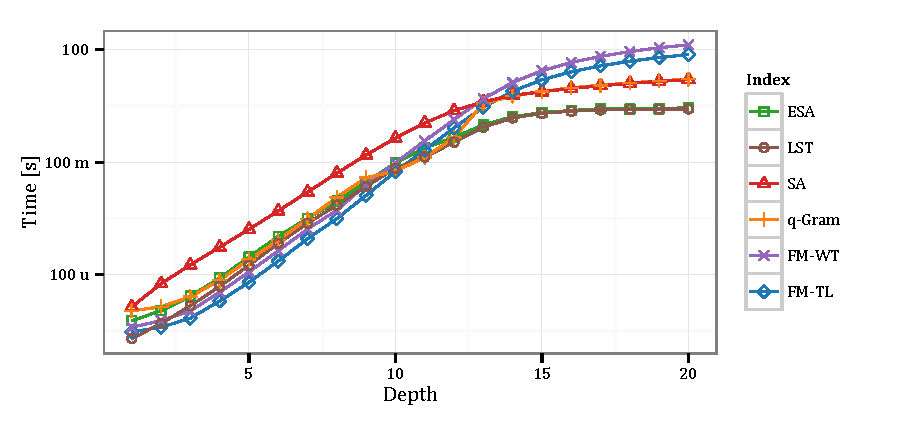
\includegraphics{visit.dna.celegans.pdf}
\end{center}
\end{figure}

\subsection{Exact string matching}
\label{sec:index:algo:exact}

I now give a simple algorithm performing exact string matching on a generic suffix trie.
In the following, I assume the text $\Text$ to be indexed by its suffix trie $\StrieOf{\Text}$.
Algorithm~\ref{alg:st-exact} searches the pattern $\Pattern$ by starting on the root node of $\StrieOf{\Text}$ and following the path spelling the pattern.
If the search ends up in a node $\StrieNode$, then each leaf $\StrieLeaf{i}$ below $\StrieNode$ points to a distinct suffix $\Suffix{\Text}{i}$ such that $\Substring{\Text}{i}{i+\Plen}$ equals $\Pattern$.
%Algorithm~\ref{alg:st-exact} is correct since each path from the root to any internal node of the suffix trie $\StrieOf{\Text}$ spells a different unique substring of $\Text$; consequently all equal substrings of $\Text$ are represented by a single common path.
If \FunctionName{goDown} is implemented in constant time and \FunctionName{occurrences} in linear time, all occurrences of $\Pattern$ into $\Text$ are found in optimal time $\Oh(\Plen+o)$, where $\Plen$ is the length of $\Pattern$ and $o$ its number of occurrences in $\Text$.

Figure \ref{fig:query-dna-exact} shows the results of the experimental evaluation of algorithm~\ref{alg:st-exact}.
On forward indices (LST, ESA, SA and $q$-gram index) the search time becomes practically constant for patterns of length above 15, \ie when the tree becomes sparse.
Conversely, on backward (FM) indices the practical search time stays linear in the pattern length. 

The ESA and LST are never faster than the $q$-gram index despite their higher memory consumption.
The SA alone is at least 20\,\% slower than the $q$-gram index, hence never competitive.
In particular, the SA shows a runtime peak for patterns of length 10, due to the fact that binary search algorithms \ref{alg:sa-lower}--\ref{alg:sa-upper} converge more slowly for shorter patterns.

\begin{figure*}[t]
\begin{center}
\begin{minipage}[t]{.8\textwidth}
\begin{algorithm}[H]
\Algorithm{ExactSearch}{$t,p$}
\begin{tabular}{ll}
\textbf{Input}  & $t$ : pointer to the root node of the suffix trie of the text\\
				& $p$ : pointer to the pattern\\
\textbf{Output} & list of all occurrences of the pattern in the text\\
\end{tabular}
\begin{algorithmic}[1]
\If {\Call{atEnd}{$p$}}
	\State \Report \Call{occurrences}{$t$}
\ElsIf {\Call{goDown}{$t,\Call{value}{p}$}}
		\State {\Call{goNext}{$p$}}
		\State \Call{ExactSearch}{$t,p$}
\EndIf
\end{algorithmic}
\label{alg:st-exact}
\end{algorithm}
\end{minipage}
\end{center}
\end{figure*}

\begin{figure}[b]
\begin{center}
\caption[Exact string matching runtime]{Runtime of exact string matching on various suffix trie implementations.}
\label{fig:query-dna-exact}
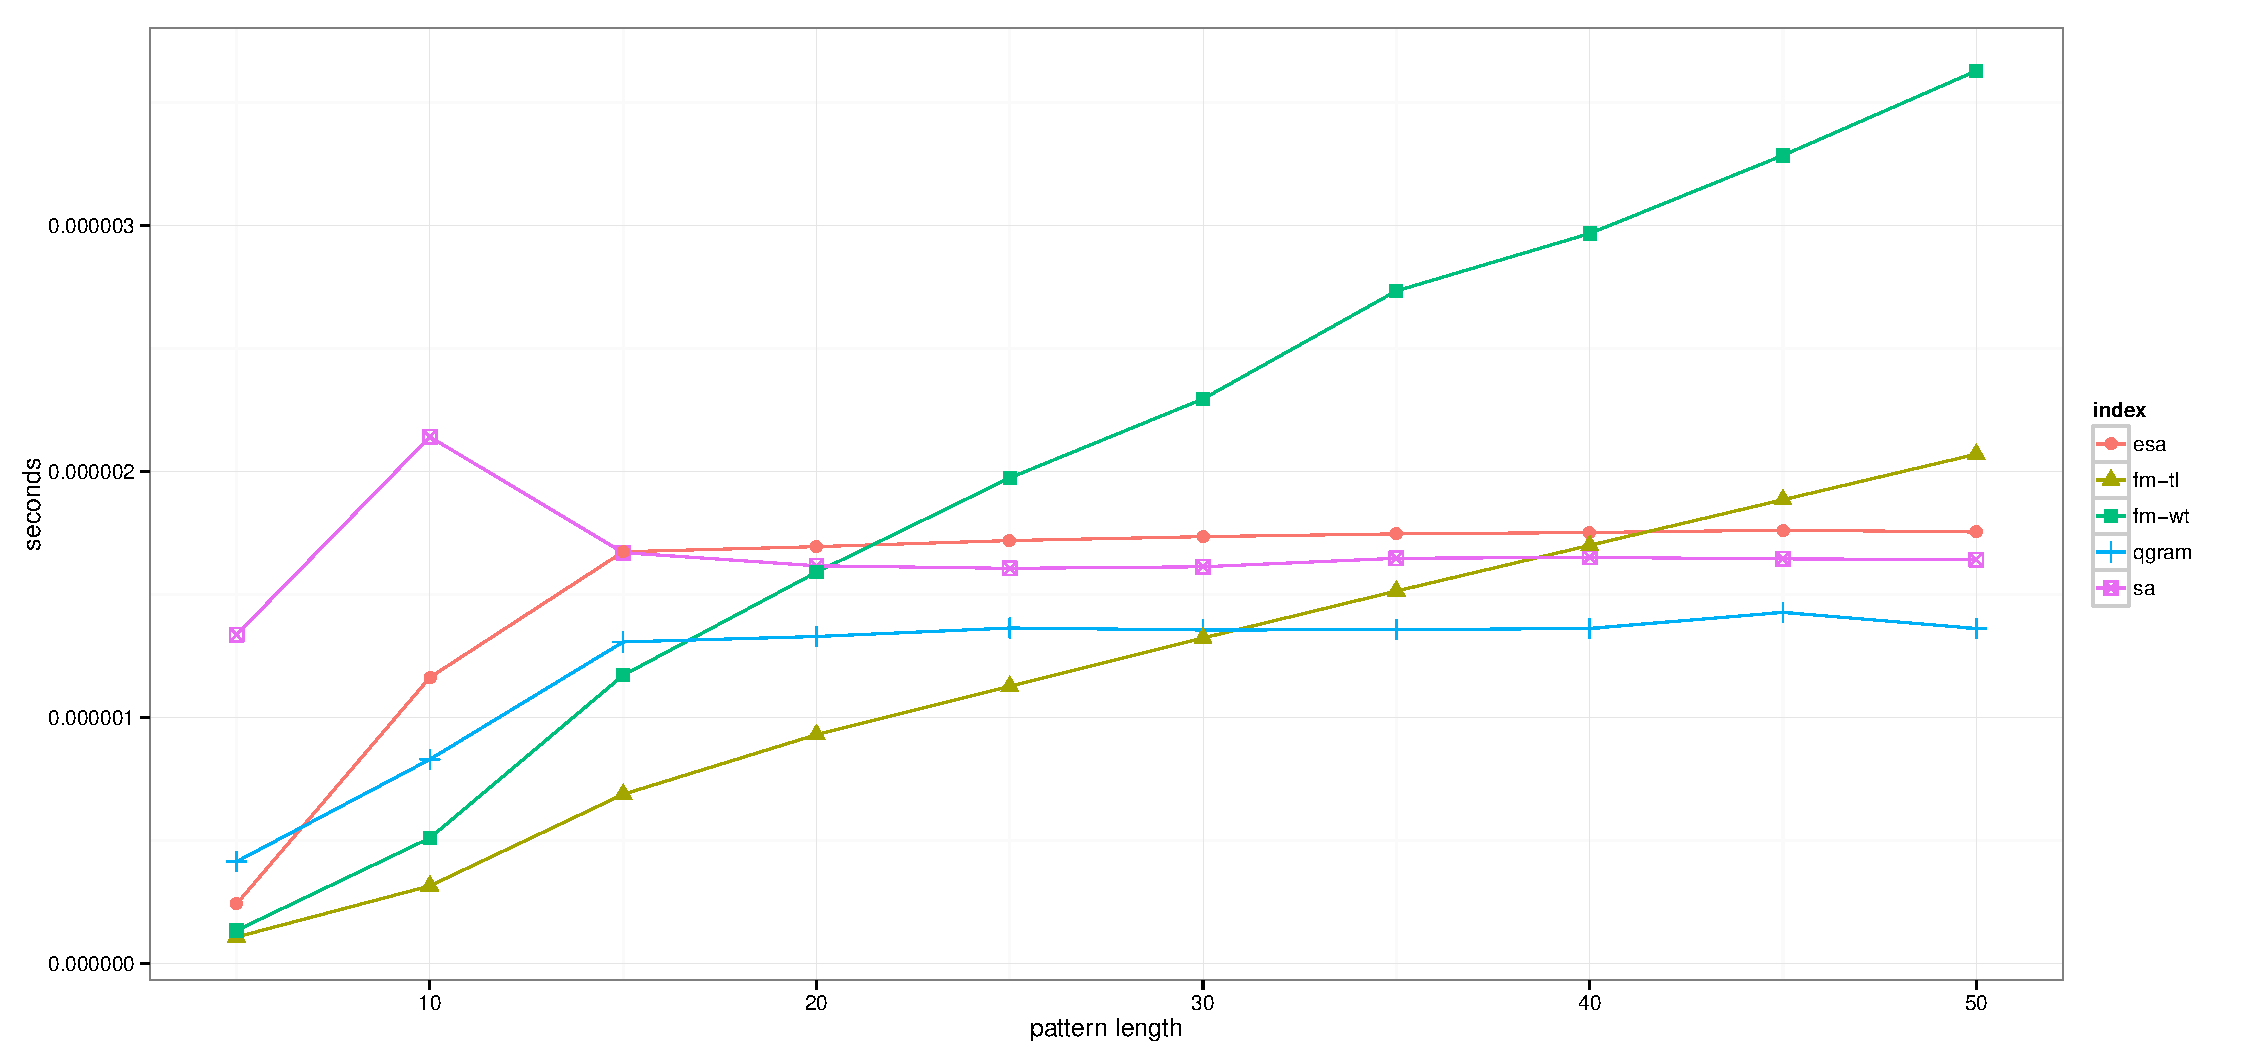
\includegraphics{query.dna.celegans.0.pdf}
\end{center}
\end{figure}


Concerning FM-indices, the WT variant is almost twice as slow as the TL variant, as the WT-based rank dictionary performs twice the number of random memory accesses than the levels rank dictionary.
Summing up, the TL FM-index is the fastest index to match exact patterns within length 30, while the $q$-gram index is the fastest for patterns above length 30.

%\begin{figure}[h]
%\begin{center}
%\caption[Exact string matching on a suffix trie]{Exact string matching on a suffix trie. The pattern NA is searched exactly in the text ANANAS\$.}
%\label{fig:st-exact}
%\begin{tikzpicture}[scale=1.5,font=\sffamily]

\tikzstyle{level 1}=[sibling distance=12mm, level distance=6mm]
\tikzstyle{level 2}=[sibling distance=6mm, level distance=6mm]
\tikzstyle{level 3}=[sibling distance=6mm, level distance=6mm] 
\tikzstyle{level 4}=[sibling distance=6mm, level distance=6mm] 
\tikzstyle{level 5}=[sibling distance=6mm, level distance=6mm] 
\tikzstyle{level 6}=[sibling distance=6mm, level distance=6mm] 
\tikzstyle{level 7}=[sibling distance=6mm, level distance=6mm] 

%\tikzstyle{transparent}=[edge from parent/.style={draw=none}]
%\tikzstyle{el}=[->,thick,color=gray,text=mycolor1high]

\tikzstyle{transparent}=[edge from parent/.style={draw=none}]
\tikzstyle{el}=[->,thick,color=black,text=black]
\tikzstyle{inner}=[circle,draw,color=black,inner sep=1.5pt]

\node[inner](r) {}
child[transparent] {
node[leaf](D) {$7$}
}
child[transparent] {
node[inner](A) {}
child[transparent] {
node[inner](AN) {}
child[transparent] {
node[inner](ANA) {}
child[transparent] {
node[inner](ANAN) {}
child[transparent] {
node[inner](ANANA) {}
child[transparent] {
node[inner](ANANAS) {}
child[transparent] {
node[leaf](ANANASD) {$1$}
}
}
}
}
child[transparent] {
node[inner](ANAS) {}
child[transparent] {
node[leaf](ANASD) {$3$}
}
}
}
}
child[transparent] {
node[inner](AS) {}
child[transparent] {
node[leaf](ASD) {$5$}
}
}
}
child[transparent] {
node[inner](N) {}
child[transparent] {
node[inner](NA) {}
child[transparent] {
node[inner](NAN) {}
child[transparent] {
node[inner](NANA) {}
child[transparent] {
node[inner](NANAS) {}
child[transparent] {
node[leaf](NANASD) {$2$}
}
}
}
}
child[transparent] {
node[inner](NAS) {}
child[transparent] {
node[leaf](NASD) {$4$}
}
}
}
}
child[transparent] {
node[inner](S) {}
child[transparent] {
node[leaf](SD) {$6$}
}
}
;

\draw[el] (r) -- (D) \labelA{\$};
\draw[el] (r) -- (A) \labelA{A};
\draw[el] (A) -- (AN) \labelA{N};
\draw[el] (AN) -- (ANA) \labelA{A};
\draw[el] (ANA) -- (ANAN) \labelA{N};
\draw[el] (ANAN) -- (ANANA) \labelA{A};
\draw[el] (ANANA) -- (ANANAS) \labelA{S};
\draw[el] (ANANAS) -- (ANANASD) \labelA{\$};
\draw[el] (ANA) -- (ANAS) \labelA{S};
\draw[el] (ANAS) -- (ANASD) \labelA{\$};
\draw[el] (A) -- (AS) \labelA{S};
\draw[el] (AS) -- (ASD) \labelA{\$};

\draw[el] (r) -- (N) \labelA{N};
\draw[el] (N) -- (NA) \labelA{A};
\draw[el] (NA) -- (NAN) \labelA{N};
\draw[el] (NAN) -- (NANA) \labelA{A};
\draw[el] (NANA) -- (NANAS) \labelA{S};
\draw[el] (NANAS) -- (NANASD) \labelA{\$};
\draw[el] (NA) -- (NAS) \labelA{S};
\draw[el] (NAS) -- (NASD) \labelA{\$};
\draw[el] (r) -- (S) \labelA{S};
\draw[el] (S) -- (SD) \labelA{\$};

\end{tikzpicture}

%\end{center}
%\end{figure}

\subsection{Backtracking $k$-mismatches}
\label{sec:index:algo:kmismatches}

I now give an algorithm that solves $k$-mismatches by backtracking a generic suffix trie.
The idea of backtracking a suffix tree has been first proposed in \citep{Ukkonen1993}.
Recently, various popular bioinformatics tools, \eg Bowtie \citep{Langmead2009} and BWA \citep{Li2009}, adopted variations of this method in conjunction with an FM-index.
Yet, the idea dates back to more than twenty years ago.

Algorithm~\ref{alg:st-hamming} performs a top-down traversal on the suffix trie $\StrieOf{\Text}$, spelling incrementally all distinct substrings of $\Text$.
While traversing each branch of the trie, this algorithm incrementally computes the distance between the query and the spelled string.
If the computed distance exceeds $k$, the traversal backtracks and proceeds on the next branch.
Conversely, if the pattern $\Pattern$ is completely spelled and the traversal ends up in a node $\StrieNode$, each leaf $\StrieLeaf{i}$ below $\StrieNode$ points to a distinct suffix $\Suffix{\Text}{i}$ such that $d_H(\Substring{\Text}{i}{i+\Plen}, \Pattern) \leq k$.

\begin{figure}[b]
\begin{center}
\caption[$k$-mismatches runtime]{Runtime of $1$-mismatch search on various suffix trie implementations.}
\label{fig:query-dna-apx}
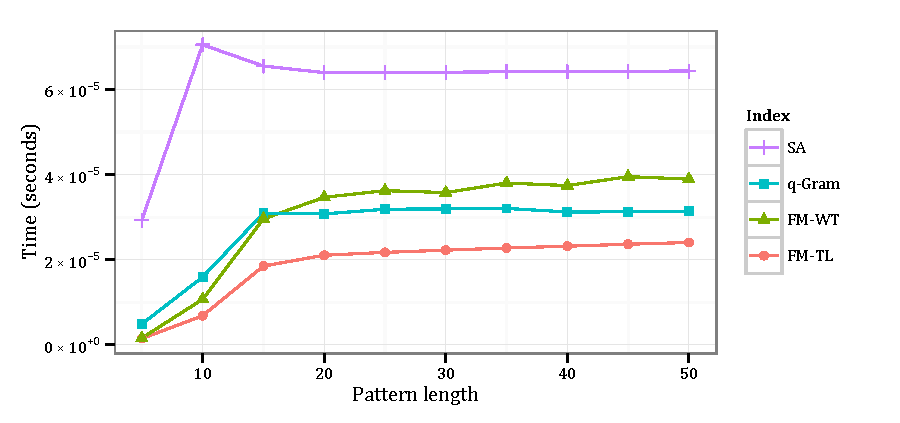
\includegraphics{query.dna.celegans.1.pdf}
\end{center}
\end{figure}

\begin{figure*}[t]
\begin{center}
\begin{minipage}[t]{.8\textwidth}
\begin{algorithm}[H]
\Algorithm{KMismatches}{$t,p,k$}
\begin{tabular}{ll}
\textbf{Input}  & $t$ : pointer to the root node of the suffix trie of the text\\
 			    & $p$ : pointer to the pattern\\
 			    & $k$ : integer bounding the number of mismatches\\
\textbf{Output} & list of all occurrences of the pattern in the text\\
\end{tabular}
\begin{algorithmic}[1]
\If {$k = 0$}
	\State {\Call{ExactSearch}{$t,p$}}
\Else
	\If {\Call{atEnd}{$p$}}
		\State \Report \Call{occurrences}{$t$}
	\ElsIf {\Call{goDown}{$t$}}
		\Repeat
			\State {$d \gets \delta(\Call{label}{t}, \Call{value}{p})$}
			\State \Call{goNext}{$p$}
			\State \Call{KMismatches}{$t,p,k - d$}
			\State \Call{goPrevious}{$p$}
		\Until \Call{goRight}{$t$}
	\EndIf
\EndIf
\end{algorithmic}
\label{alg:st-hamming}
\end{algorithm}
\end{minipage}
\end{center}
\end{figure*}

%The \emph{worst case} runtime of algorithm \ref{alg:st-hamming} is clearly independent of the text length $\Tlen$.
%According to \citep{Navarro2000}, this algorithm exhibits average time sublinear in $\Tlen$.

%\begin{figure}[h]
%\begin{center}
%\caption[Backtracking $k$-mismatches]{$k$-mismatches on a suffix trie.}
%\label{fig:st-hamming}
%\begin{tikzpicture}[scale=1.5,font=\sffamily]

\tikzstyle{level 1}=[sibling distance=12mm, level distance=6mm]
\tikzstyle{level 2}=[sibling distance=6mm, level distance=6mm]
\tikzstyle{level 3}=[sibling distance=6mm, level distance=6mm] 
\tikzstyle{level 4}=[sibling distance=6mm, level distance=6mm] 
\tikzstyle{level 5}=[sibling distance=6mm, level distance=6mm] 
\tikzstyle{level 6}=[sibling distance=6mm, level distance=6mm] 
\tikzstyle{level 7}=[sibling distance=6mm, level distance=6mm] 

%\tikzstyle{transparent}=[edge from parent/.style={draw=none}]
%\tikzstyle{el}=[->,thick,color=gray,text=mycolor1high]

\tikzstyle{transparent}=[edge from parent/.style={draw=none}]
\tikzstyle{el}=[->,thick,color=black,text=black]
\tikzstyle{inner}=[circle,draw,color=black,inner sep=1.5pt]

\node[inner](r) {}
child[transparent] {
node[leaf](D) {$7$}
}
child[transparent] {
node[inner](A) {}
child[transparent] {
node[inner](AN) {}
child[transparent] {
node[inner](ANA) {}
child[transparent] {
node[inner](ANAN) {}
child[transparent] {
node[inner](ANANA) {}
child[transparent] {
node[inner](ANANAS) {}
child[transparent] {
node[leaf](ANANASD) {$1$}
}
}
}
}
child[transparent] {
node[inner](ANAS) {}
child[transparent] {
node[leaf](ANASD) {$3$}
}
}
}
}
child[transparent] {
node[inner](AS) {}
child[transparent] {
node[leaf](ASD) {$5$}
}
}
}
child[transparent] {
node[inner](N) {}
child[transparent] {
node[inner](NA) {}
child[transparent] {
node[inner](NAN) {}
child[transparent] {
node[inner](NANA) {}
child[transparent] {
node[inner](NANAS) {}
child[transparent] {
node[leaf](NANASD) {$2$}
}
}
}
}
child[transparent] {
node[inner](NAS) {}
child[transparent] {
node[leaf](NASD) {$4$}
}
}
}
}
child[transparent] {
node[inner](S) {}
child[transparent] {
node[leaf](SD) {$6$}
}
}
;

\draw[el] (r) -- (D) \labelA{\$};
\draw[el] (r) -- (A) \labelA{A};
\draw[el] (A) -- (AN) \labelA{N};
\draw[el] (AN) -- (ANA) \labelA{A};
\draw[el] (ANA) -- (ANAN) \labelA{N};
\draw[el] (ANAN) -- (ANANA) \labelA{A};
\draw[el] (ANANA) -- (ANANAS) \labelA{S};
\draw[el] (ANANAS) -- (ANANASD) \labelA{\$};
\draw[el] (ANA) -- (ANAS) \labelA{S};
\draw[el] (ANAS) -- (ANASD) \labelA{\$};
\draw[el] (A) -- (AS) \labelA{S};
\draw[el] (AS) -- (ASD) \labelA{\$};

\draw[el] (r) -- (N) \labelA{N};
\draw[el] (N) -- (NA) \labelA{A};
\draw[el] (NA) -- (NAN) \labelA{N};
\draw[el] (NAN) -- (NANA) \labelA{A};
\draw[el] (NANA) -- (NANAS) \labelA{S};
\draw[el] (NANAS) -- (NANASD) \labelA{\$};
\draw[el] (NA) -- (NAS) \labelA{S};
\draw[el] (NAS) -- (NASD) \labelA{\$};
\draw[el] (r) -- (S) \labelA{S};
\draw[el] (S) -- (SD) \labelA{\$};

\end{tikzpicture}

%\end{center}
%\end{figure}

Figure \ref{fig:query-dna-apx} shows the results of the experimental evaluation of algorithm~\ref{alg:st-hamming} for $k=1$.
The TL FM-index is always faster than any other index: for instance, on patterns of length 30, the SA is 3 times slower; even the $q$-gram index is 50\,\% slower than the TL FM-index.
Despite their tree structure, ESA and LST are always slower than $q$-gram and FM-indices.

On the TL FM-index, $1$-approximate matching of patterns of length 30 is 16 times slower than exact matching: on average, $1$-approximate matching spends $21$ microseconds ($\mu s$), while exact matching takes $1.3 \, \mu s$.
On the ESA, $1$-approximate matching shows a slow-down of 24 times: $1$-approximate matching spends $40.8 \, \mu s$, compared to the $1.7 \, \mu s$ for exact matching.

%\subsection{Backtracking $k$-differences}
%\label{sec:index:algo:kdifferences}
%
%I present two alternative algorithms for $k$-differences.
%Algorithm~\ref{alg:st-edit-explicit} explicitly enumerates errors while traversing the suffix trie. Conversely, algorithm~\ref{alg:st-edit} computes the edit distance between the pattern and any branch of the suffix trie.
%This latter algorithm necessitates of a method capable of checking incrementally whether the edit distance at any node is within the imposed threshold $k$.
%
%%Algorithm~\ref{alg:st-edit-explicit} reports more occurrences than algorithm~\ref{alg:st-edit}.
%%Discuss neighborhood, condensed neighborhood, and super-condensed neighborhood.
%%To obtain a better theoretical runtime, \citep{Navarro2000} consider an algorithm that computes in $\Oh(1)$ per node.
%
%\begin{figure*}[b]
%\begin{center}
%\begin{minipage}[t]{.8\textwidth}
%\begin{algorithm}[H]
%\Algorithm{KDifferences}{$t,p,e$}
%\begin{tabular}{ll}
%\textbf{Input}  & $t$ : pointer to the root node of the suffix trie of the text\\
% 			    & $p$ : pointer to the root node of the trie of the patterns\\
% 			    & $e$ : integer bounding the number of errors\\
%\textbf{Output} & list of all occurrences of the pattern in the text\\
%\end{tabular}
%\begin{algorithmic}[1]
%\If {$e = k$}
%	\State \Call{ExactSearch}{$t,p$}
%\Else
%	\State \Call{goNext}{$p$}
%	\State \Call{KDifferences}{$t,p,e+1$}
%	\State \Call{goPrevious}{$p$}
%	\If {\Call{goDown}{$t$}}
%		\Repeat
%			\State \Call{KDifferences}{$t,p,e+1$}
%			\State {$d \gets \delta(\Call{label}{t}, \Call{value}{p})$}
%			\State \Call{goNext}{$p$}
%			\State \Call{KDifferences}{$t,p,e + d$}
%			\State \Call{goPrevious}{$p$}
%		\Until {\Call{goRight}{$t$}}
%	\EndIf
%\EndIf
%\end{algorithmic}
%\label{alg:st-edit-explicit}
%\end{algorithm}
%\end{minipage}
%\end{center}
%\end{figure*}
%
%\begin{figure*}[b]
%\begin{center}
%\begin{minipage}[t]{.8\textwidth}
%\begin{algorithm}[H]
%\Algorithm{KDifferences}{$t,p,D$}
%\begin{tabular}{ll}
%\textbf{Input}  & $t$ : pointer to the root node of the suffix trie of the text\\
% 			    & $p$ : pointer to the root node of the trie of the patterns\\
% 			    & $D$ : vector of integers representing a DP column\\
%\textbf{Output} & list of all occurrences of the pattern in the text\\
%\end{tabular}
%\begin{algorithmic}[1]
%\If {$D[m] \leq k$}
%	\State \Report \Call{occurrences}{$t$}
%\ElsIf {$\min{D} \leq k$}
%	\If {\Call{goDown}{$t$}}
%		\Repeat
%			\State {$D' \gets$ \Call{DP}{$D, \Call{label}{t}, p$}}
%			\State \Call{goNext}{$p$}
%			\State \Call{KDifferences}{$t,p,D'$}
%			\State \Call{goPrevious}{$p$}
%		\Until {\Call{goRight}{$t$}}
%	\EndIf
%\EndIf
%\end{algorithmic}
%\label{alg:st-edit}
%\end{algorithm}
%\end{minipage}
%\end{center}
%\end{figure*}
%
%%\begin{algorithm}[h]
%%\caption{$k$-difference on a suffix trie.}
%%\label{alg:st-edit}
%%\begin{algorithmic}[1]
%%\Procedure{KDifferences}{$\StrieNode,p,e$}
%%	\ForAll {$\StrieChar \in \Ci(\StrieNode)$}
%%		\State \Call{KDifferences}{$\StrieChar,p_{2..|p|},e - d_E(repr(\StrieNode), p)$}
%%	\EndFor
%%\EndProcedure
%%\end{algorithmic}
%%\end{algorithm}


\subsection{Multiple exact string matching}
\label{sec:index:algo:multiexact}

Before turning to multiple $k$-mismatches, I describe a simpler algorithm for multiple exact string matching.
In addition to the text $\Text$, multiple exact string matching provides a collection of patterns $\Patterns$.
Hence, in addition to the suffix trie $\StrieOf{\Text}$, algorithm \ref{alg:st-exact-multi} considers the trie $\RtrieOf{\Patterns}$.
Algorithm \ref{alg:st-exact-multi} matches simultaneously in $\StrieOf{\Text}$ all patterns indexed in $\RtrieOf{\Patterns}$.
The traversal performed by algorithm \ref{alg:st-exact-multi} visits pairs of nodes in $\StrieOf{\Text} \times \RtrieOf{\Patterns}$ whose entering edges have the same label.
Such traversal implicitly \emph{intersects} the two tries.
However, algorithm \ref{alg:st-exact-multi} is not symmetric: $\StrieOf{\Text}$ and $\RtrieOf{\Patterns}$ cannot be interchanged.
The traversal stops whenever it reaches a leaf node in $\RtrieOf{\Patterns}$ and reports the occurrences pointed by all the leaves beneath the current node in $\StrieOf{\Text}$.
%If the collection $\Patterns$ contains two equal strings, some leaf of $\Patterns$ points to more than one pattern.

\begin{figure*}[t]
\begin{center}
\begin{minipage}[t]{.8\textwidth}
\begin{algorithm}[H]
\Algorithm{MultipleExactSearch}{$t,p$}
\begin{tabular}{ll}
\textbf{Input}  & $t$ : pointer to the root node of the suffix trie of the text\\
 			    & $p$ : pointer to the root node of the trie of the patterns\\
\textbf{Output} & list of all occurrences of any pattern in the text\\
\end{tabular}
\begin{algorithmic}[1]
\If {\Call{isLeaf}{$p$}}
	\State \Report \Call{occurrences}{$t$} $\times$ \Call{occurrences}{$p$}
\Else
	\State \Call{goDown}{$p$}
	\Repeat
		\If {\Call{goDown}{$t, \Call{label}{p}$}}
			\State \Call{MultipleExactSearch}{$t,p$}
			\State \Call{goUp}{$t$}
		\EndIf
	\Until {\Call{goRight}{$p$}}
\EndIf
\end{algorithmic}
\label{alg:st-exact-multi}
\end{algorithm}
\end{minipage}
\end{center}
\end{figure*}

\begin{figure}[b]
\begin{center}
\caption[Multiple exact string matching runtime]{Runtime of multiple exact string matching on various suffix trie implementations. Pattern length is fixed to 15. Preprocessing times are shown in black.}
\label{fig:query-dna-exact-multi}
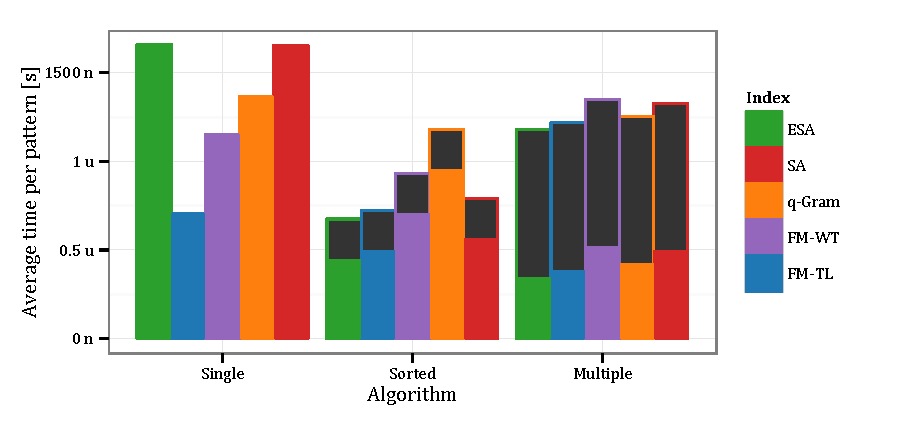
\includegraphics{multi.dna.celegans.0.15.pdf}
\end{center}
\end{figure}

The experimental evaluation compares algorithm~\ref{alg:st-exact-multi} (Multiple) with algorithm~\ref{alg:st-exact} processing patterns in random order (Single) and in lexicographic order (Sorted).
Figure~\ref{fig:query-dna-exact-multi} shows the results.
These three methods ran on 10~M patterns of length 30: runtimes shown in figure \ref{fig:query-dna-exact-multi} (histogram Single) correspond to runtimes shown in figure \ref{fig:query-dna-exact} (plots at pattern length 15).
%For instance, the indices ranked by query speed are: TL FM-index, WT FM-index, $q$-gram index, ESA and SA.

Figure \ref{fig:query-dna-exact-multi} shows that a simple lexicographical sort of the patterns (histogram Sorted) speeds up algorithm \ref{alg:st-exact} on the SA and ESA by a factor of 2.
The same trick does not yield a significant speed-up on FM-indices nor on the $q$-gram index, as the $q$-gram directory already provides a cache local access pattern.

Algorithm~\ref{alg:st-exact-multi} (histogram Multiple) further reduces the traversal time.
Nonetheless, its runtime is dominated by the additional preprocessing time paid to construct the trie of the patterns.
This algorithm becomes more useful as a primitive within the multiple $k$-mismatches algorithm, presented in the following section.

\subsection{Multiple $k$-mismatches}
\label{sec:index:algo:multimismatch}

Algorithm \ref{alg:st-hamming-multi} is the straightforward generalization of algorithm \ref{alg:st-exact-multi} to $k$-mismatches.
The algorithm receives a collection of patterns $\Patterns$ and performs backtracking on $\Texts$ as in algorithm  \ref{alg:st-hamming}, this time using the associated trie $\Patterns$.

\begin{figure*}[t]
\begin{center}
\begin{minipage}[t]{.8\textwidth}
\begin{algorithm}[H]
\Algorithm{MultipleKMismatches}{$t,p,k$}
\begin{tabular}{ll}
\textbf{Input}  & $t$ : pointer to the root node of the suffix trie of the text\\
 			    & $p$ : pointer to the root node of the trie of the patterns\\
 			    & $k$ : integer bounding the number of mismatches\\
\textbf{Output} & list of all occurrences of any pattern in the text\\
\end{tabular}
\begin{algorithmic}[1]
\If {$k = 0$}
	\State {\Call{MultipleExactSearch}{$t,p$}}
\Else
	\If {\Call{isLeaf}{$p$}}
		\State \Report \Call{occurrences}{$t$} $\times$ \Call{occurrences}{$p$}
	\ElsIf {\Call{goDown}{$t$}}
		\Repeat
			\State {\Call{goDown}{$p$}}
			\Repeat
				\State {$d \gets \delta(\Call{label}{t}, \Call{label}{p})$}
				\State \Call{MultipleKMismatches}{$t,p,k-d$}
			\Until {\Call{goRight}{$p$}}
			\State {\Call{goUp}{$p$}}
		\Until {\Call{goRight}{$t$}}
	\EndIf
\EndIf
\end{algorithmic}
\label{alg:st-hamming-multi}
\end{algorithm}
\end{minipage}
\end{center}
\end{figure*}

The experimental evaluation compares algorithm~\ref{alg:st-hamming-multi} (Multiple) with algorithm~\ref{alg:st-hamming} processing patterns in random order (Single) and in lexicographic order (Sorted).
All three methods ran on 10~M patterns of length 30, with $k$ fixed to 1.
Thus, runtimes shown in figure \ref{fig:query-dna-apx-multi} (histogram Single) correspond to runtimes shown in figure \ref{fig:query-dna-apx} (plots at pattern length 30).

\begin{figure}[b]
\begin{center}
\caption[Multiple $k$-mismatches runtime]{Runtime of multiple $1$-mismatch on various suffix trie implementations. Pattern length is fixed to 30. Preprocessing times are shown in black.}
\label{fig:query-dna-apx-multi}
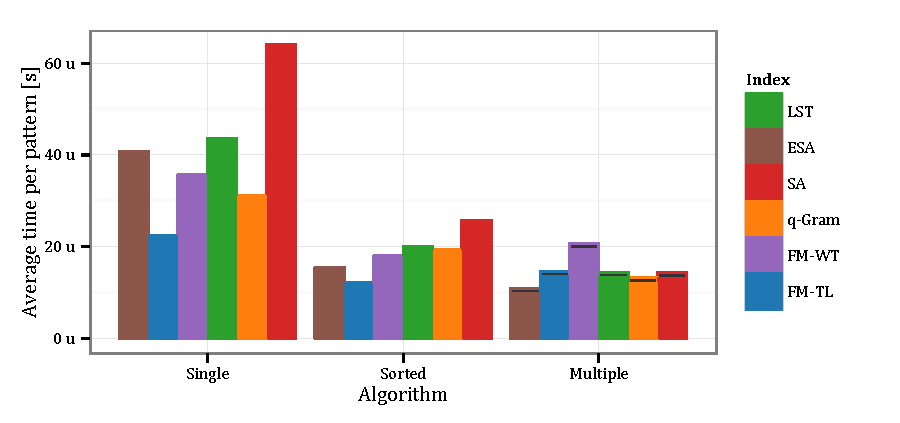
\includegraphics{multi.dna.celegans.1.30.pdf}
\end{center}
\end{figure}

Algorithm \ref{alg:st-hamming} on lexicographically sorted patterns (histogram Sorted) is faster by a factor of 2 or more, on all indices.
The time to sort the patterns becomes insignificant compared to the traversal time.
Algorithm \ref{alg:st-exact-multi} (histogram Multiple) reduces traversal time by a factor of 4--5 on LST, ESA, and SA.
Thus, the time to construct the trie of the patterns is easily justified.
In practice, algorithm \ref{alg:st-exact-multi} fills the gap between the runtime of the SA and the $q$-gram index.
Surprisingly, algorithm \ref{alg:st-exact-multi} increases traversal time on FM-indices.

This algorithms works according to a \emph{cache-friendly} memory access pattern, which holds for forward search but not for backward search.
Using forward search, the traversal of a suffix trie becomes less expensive as it proceeds towards bottom nodes.
Indeed, traversal towards a child node involves the computation of a subinterval of the current suffix array interval; such computation accesses memory locations within the current interval, having good chances to be in the cache.
Conversely, using backward search, the traversal becomes more expensive as it proceeds deeper in the trie; traversal downwards involves the computation of intervals outside of the current one, unlikely to be in the cache as they are accessed less often than top intervals.
Multiple backtracking factorizes the traversal of top nodes, thus it pays off with forward search rather than with backward search.

Figure \ref{fig:query-dna-apx-multi-sa} shows the average runtime of the three approaches on the SA by varying the number of patterns.
While the average runtime of the single method is constant, both multiple methods clearly benefit from receiving a higher number of patterns.
In particular, method Multiple is constantly faster than Sorted, and the runtime gap increases with the number of patterns.
The speed-up of multiple methods slowly decreases, though there is still some space of improvement with more than 10~M patterns.

Figure \ref{fig:query-dna-apx-multi-fmtl} presents the same evaluation of figure \ref{fig:query-dna-apx-multi-sa}, but for the TL FM-index.
Multiple methods exhibit again decreasing average runtimes by number of patterns.
However, here method Sorted is constantly faster than Multiple, but the runtime gap decreases with the number of patterns.
Moreover, the speed-up of both multiple methods slowly increases with the number of patterns instead of decreasing.

\begin{figure}[t]
\begin{center}
\caption[Multiple $k$-mismatches speed-up on SA]{Speed-up of multiple $1$-mismatch by number of patterns on the SA. Pattern length is fixed to 30. Traversal times without preprocessing are shown by dashed lines.}
\label{fig:query-dna-apx-multi-sa}
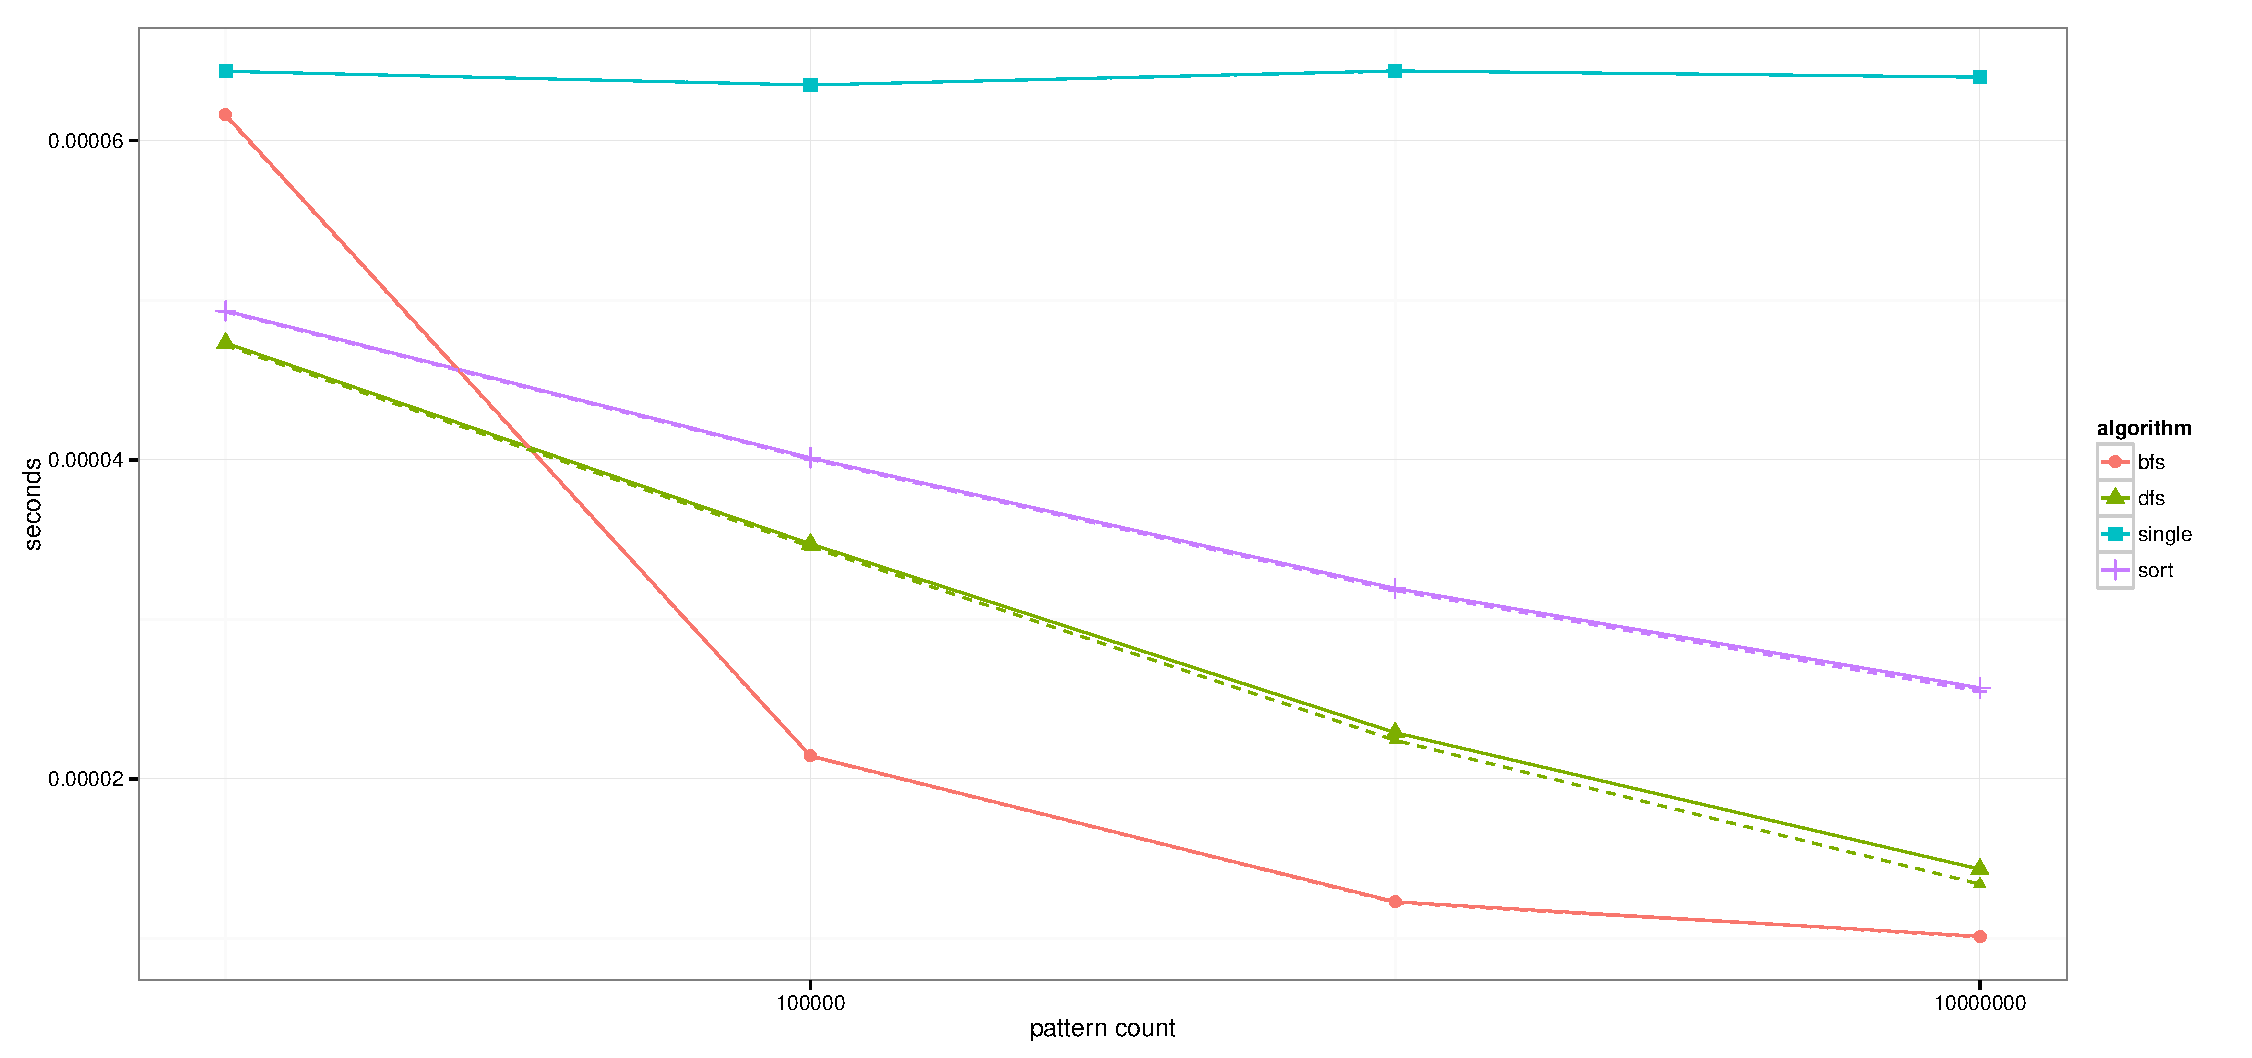
\includegraphics{multi.dna.celegans.1.sa.pdf}
\end{center}
\end{figure}

\begin{figure}[b]
\begin{center}
\caption[Multiple $k$-mismatches speed-up on FM-index]{Speed-up of multiple $1$-mismatch by number of patterns on the TL FM-Index. Pattern length is fixed to 30. Traversal times without preprocessing are shown by dashed lines.}
\label{fig:query-dna-apx-multi-fmtl}
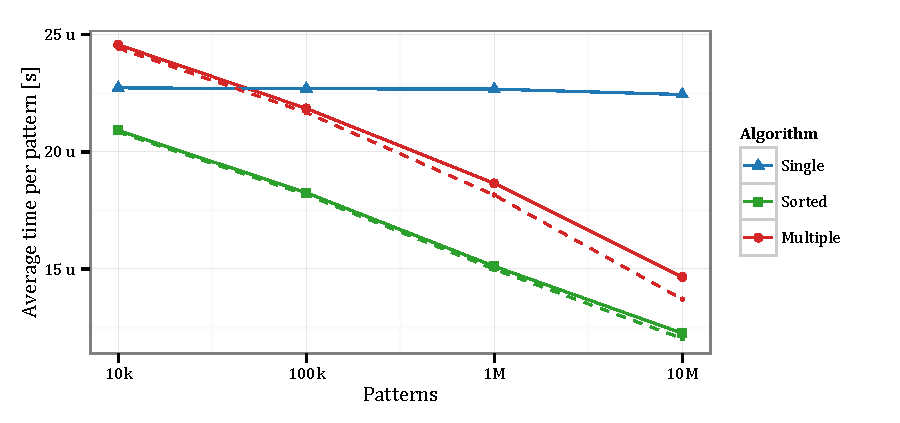
\includegraphics{multi.dna.celegans.1.fm-tl.pdf}
\end{center}
\end{figure}
